%!TEX TS-program = pdflatexmk
\documentclass[10pt]{beamer}

%packages
\usepackage{amsmath,amsthm,amssymb,amsfonts,amsxtra,amstext}
\usepackage{graphicx,float}
\usepackage{hyperref}
\usepackage{array}
\usepackage{url}
\usepackage{movie15}
\usepackage[T1]{fontenc}

\newcommand{\R}{\mathbf{r}}
\newcommand{\Rd}{\mathbf{\dot{r}}}
\newcommand{\Z}{\mathbf{z}}
\newcommand{\X}{\mathbf{x}}
\newcommand{\ang}{\mathbf{L}}
\newcommand{\ec}{\mathbf{e}}
\newcommand{\bc}{\mathbf{b}}
\def\mf{\mathbf}
\def\mc{\mathcal}
\newcommand{\leftexp}[2]{{\vphantom{#2}}^{#1}\!{#2}}
\newcommand{\fddt}[1]{\ensuremath{\leftexp{\mathcal{#1}}{\frac{\mathrm{d}}{\mathrm{d}t}}}}
\newcommand{\PSF}{\mathrm{PSF}}
\newcommand{\fdddt}[1]{\ensuremath{\leftexp{\mathcal{#1}}{\frac{\mathrm{d}^2}{\mathrm{d}t^2}}}}
\newcommand{\intd}[1]{\ensuremath{\,\mathrm{d}#1}}
\definecolor{MyBlue}{cmyk}{0.88, 0.7637,0.0032,0} 
\definecolor{MyRed}{cmyk}{0,0.994,1,0} 
\definecolor{MyGreen}{cmyk}{0.8985,0.3258,1,0.2429} 
\definecolor{MyPurple}{cmyk}{0.7708,0.847,0,0} 
\definecolor{MyGraphite}{cmyk}{0.5973,0.5124,0.5077,0.2013} 

%presentation theme
\usetheme[secheader]{Madrid}
\usecolortheme{seagull}
\usefonttheme[]{serif}

%university logo
\pgfdeclareimage[height=0.5cm]{university-logo}{PrincetonShield}
\logo{\pgfuseimage{university-logo}}

\newcommand\BackgroundPicture[3]{%
    \setbeamertemplate{background}{%
    \parbox[c][\paperheight]{\paperwidth}{%
        \vfill \hfill
 \includegraphics[width=#2\paperwidth,height=#3\paperheight]{#1}
         \hfill \vfill
      }}}

% presentation descriptors
\title[Exosystem Modeling]{Exosystem Modeling for\\ Mission Simulation and Survey Analysis}
\subtitle{Final Public Oral}
\author[Dmitry Savransky]{Dmitry Savransky}
\institute[Princeton Univ.] 
{
  Department of Mechanical and Aerospace Engineering\\
  Princeton University}
\date[06.14.2011]{June 14th, 2011}
\subject{Talks}

\begin{document}
\setbeamerfont{smalleq}{size=\small} 

\part{Talk}
\frame{\titlepage}

\section{Introduction and Background}
\subsection*{Motivation}

\BackgroundPicture{exoplan_bckgnd}{1}{1}
\frame{
\frametitle{Why Study Exoplanets?}
\textbf{
\begin{itemize}
\item Without other examples, we have only one sample of planetary systems
\item Need exoplanet observations to formulate and test planet formation and development models
\item Observing systems at other points in their development will help explain our own solar system
\item We may find life
\end{itemize}
}}
\setbeamertemplate{background}{ \setbeamercolor{normal text}{bg=white} }


\frame{
\frametitle{The Problem}
\begin{itemize}
\item Planet observations occur at the absolute boundaries of existing instrument capabilities
\item Dedicated planet-finding instruments are large, complicated, and very expensive
\item Even a perfectly functioning exoplanet observatory may not find anything
\end{itemize}

\bigskip

\begin{block}{}
\centering We need to model both exosystems and instruments to ensure that useful data will be collected and the maximum amount of information extracted.
\end{block}
}

\frame{
\frametitle{Goal}
\begin{figure}
	\begin{center}
	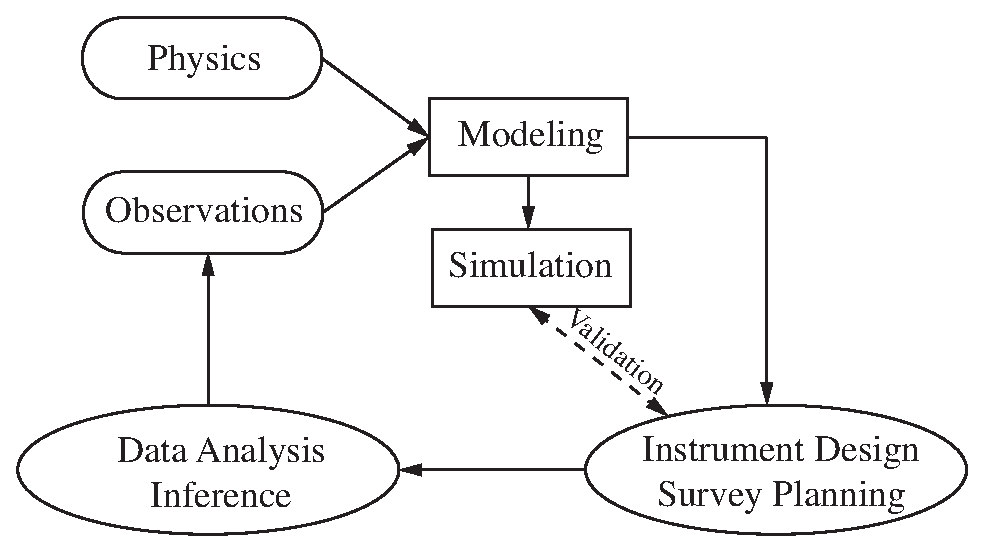
\includegraphics[width = 0.85\columnwidth]{flowchart1}
	\end{center}
\end{figure}
}

\subsection*{}
\frame{\frametitle{Outline}\tableofcontents}

\subsection{Known Exoplanets}
\frame{
\frametitle{A Brief History of Exoplanet Exploration}
\begin{figure}[ht]
\includemovie[
  controls,
  toolbar,
  poster,
  autoclose,
  text={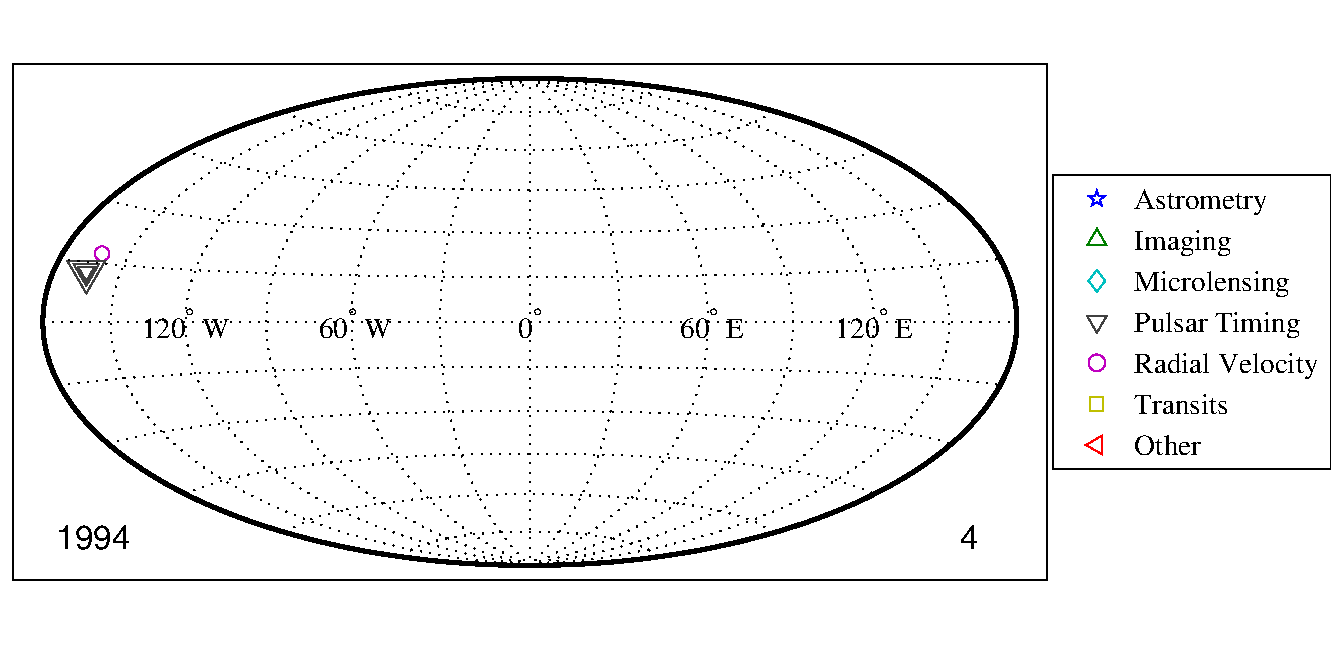
\includegraphics[scale=0.48]{exoplanetHistory_front}}
]{}{}{exoplanetHistory.mp4}
\end{figure}
}

\subsection{Planet Finding Methods}

\frame{
\frametitle{Planet-Finding Techniques Illustrated}
\begin{figure}[ht]
\includemovie[
  controls,
  toolbar,
  poster,
  text={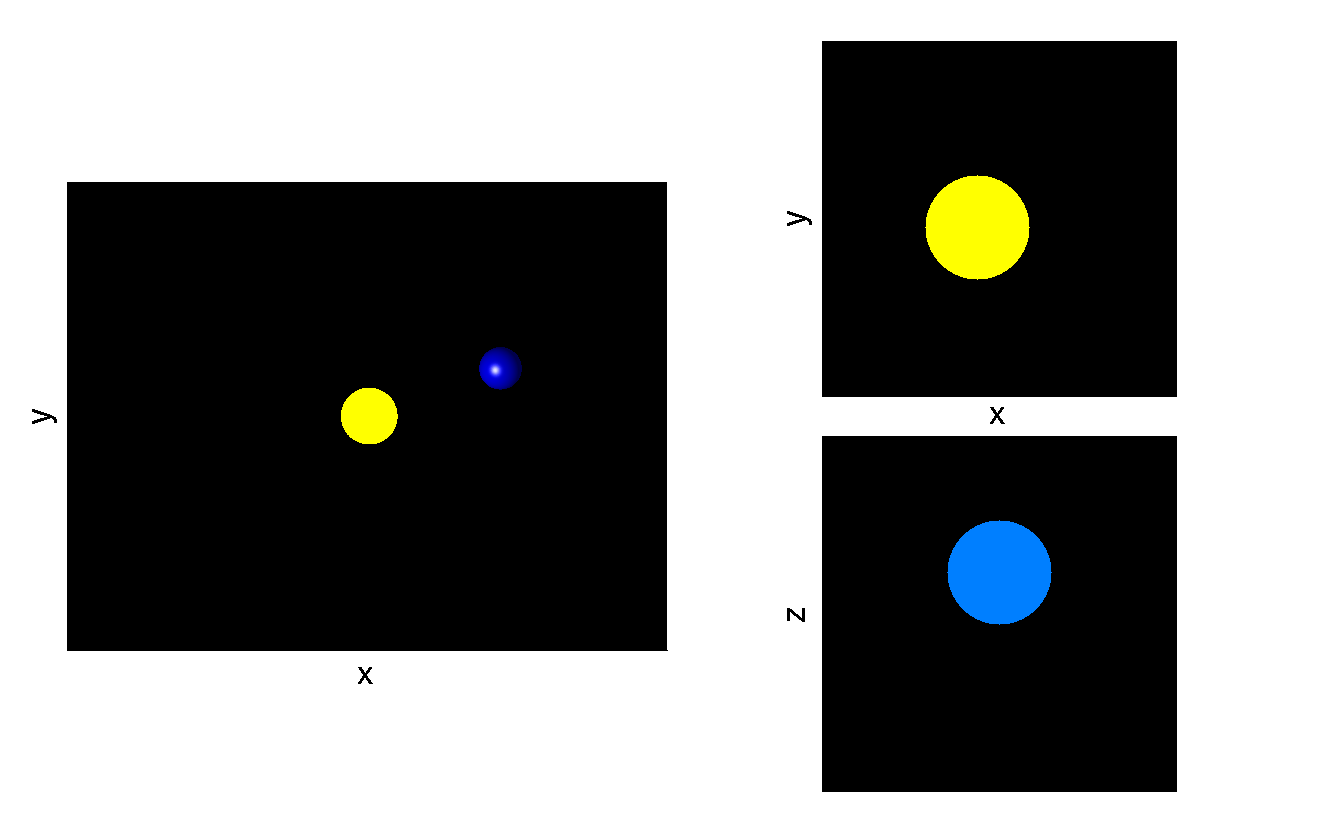
\includegraphics[width=0.75\columnwidth]{methods_anim2_front}}
]{}{}{methods2.mp4}
\end{figure}
}

\frame{
\frametitle{Exoplanet Data Sets}
\begin{columns}[c]
\column{0.5\columnwidth}
\begin{figure}[ht]
\centering
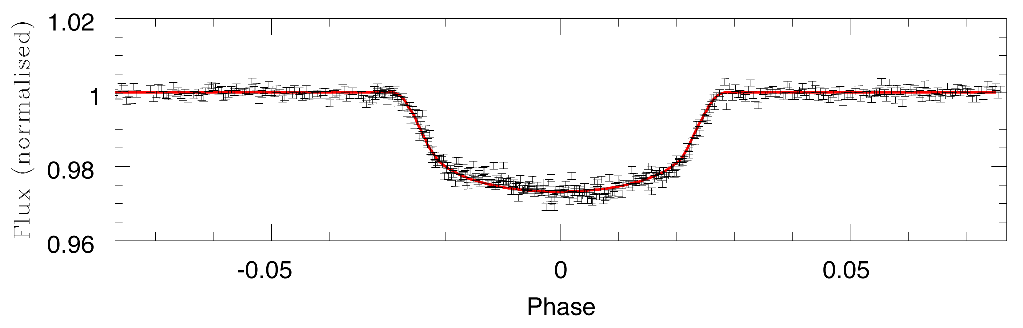
\includegraphics[width = 0.75\columnwidth]{phot_data}
\vspace{-1ex}
\caption{\cite{gillon2006high}}
\end{figure}
\vspace{-4ex}
\begin{figure}[ht]
\centering
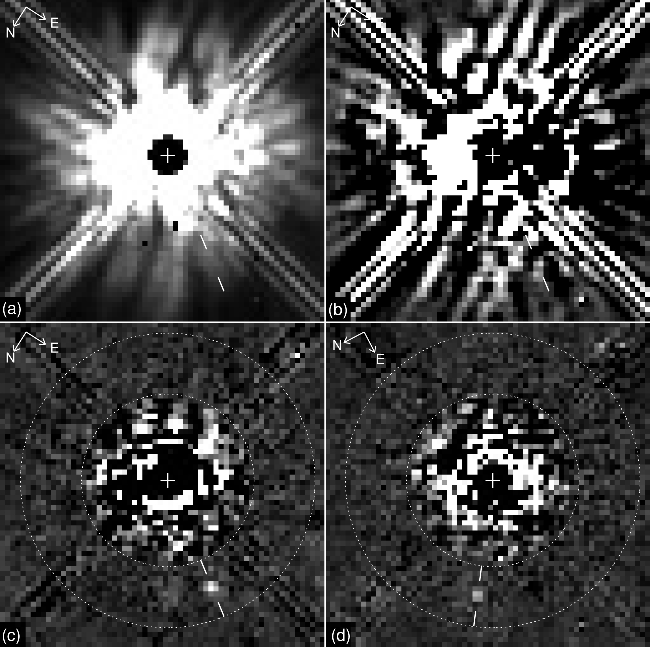
\includegraphics[width = 0.65\columnwidth]{dd_data}
\vspace{-1ex}
\caption{\cite{lafreniere2009hst}}
\end{figure}

\column{0.5\columnwidth}
\begin{figure}[ht]
\centering
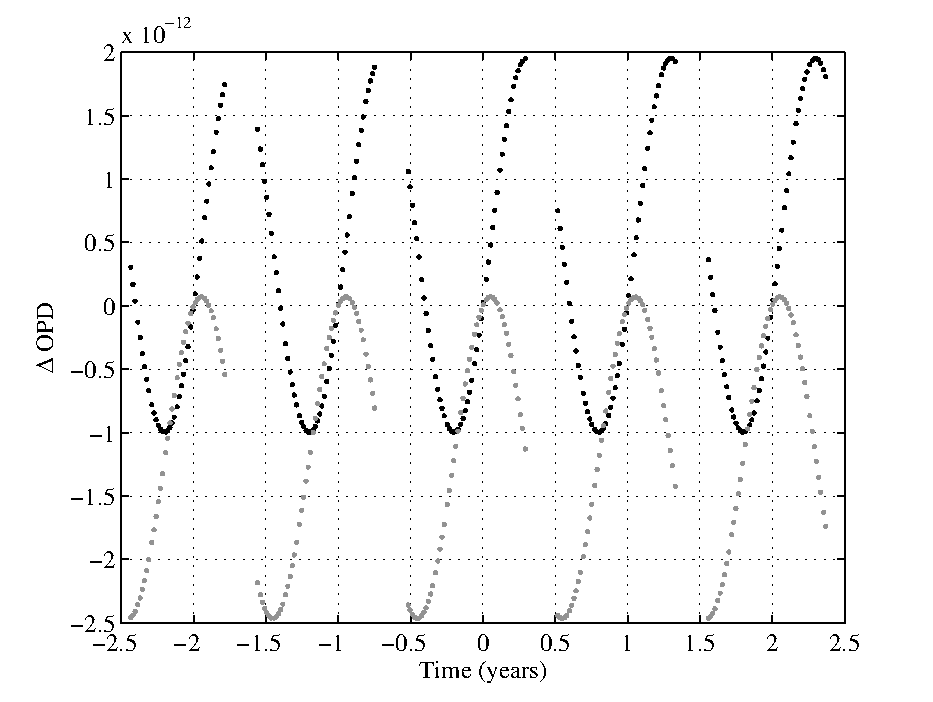
\includegraphics[width = 0.65\columnwidth]{../figures/planet_effects}
\vspace{-1ex}
\caption{Simulation}
\end{figure}
\vspace{-5ex}
\begin{figure}[ht]
\centering
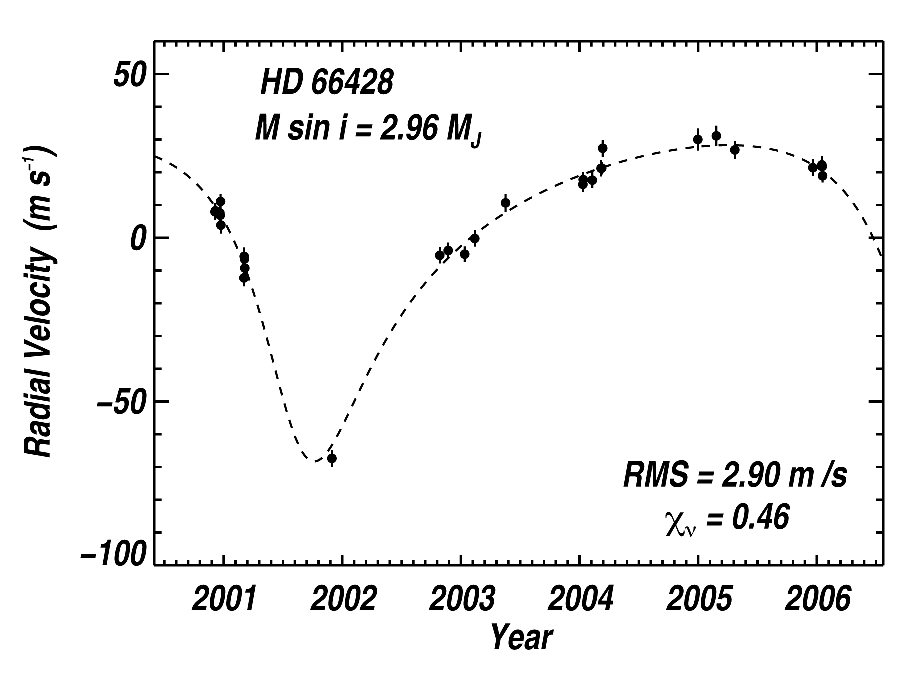
\includegraphics[width = 0.65\columnwidth]{rv_data}
\vspace{-2ex}
\caption{\cite{butler2006}}
\end{figure}

\end{columns}
}

\frame{
\frametitle{Imaging Constraints}
\begin{figure}
	\begin{center}
	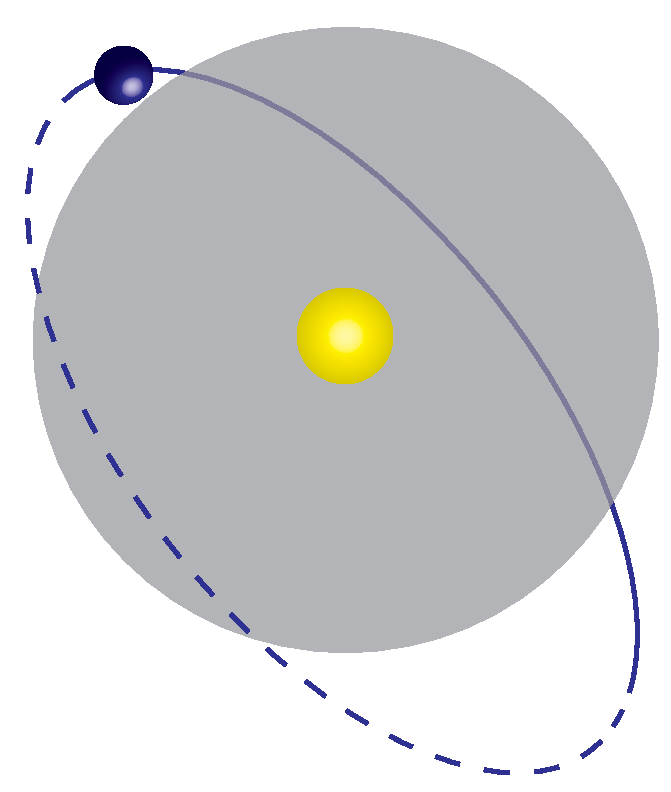
\includegraphics[width=0.3\columnwidth]{imagingConstraintsSchema}
	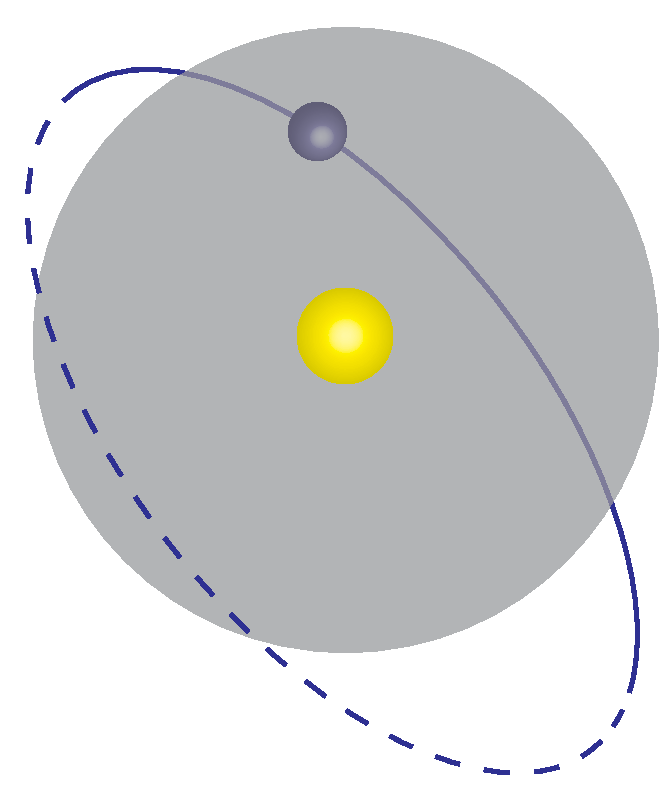
\includegraphics[width=0.3\columnwidth]{imagingConstraintsSchemb}
	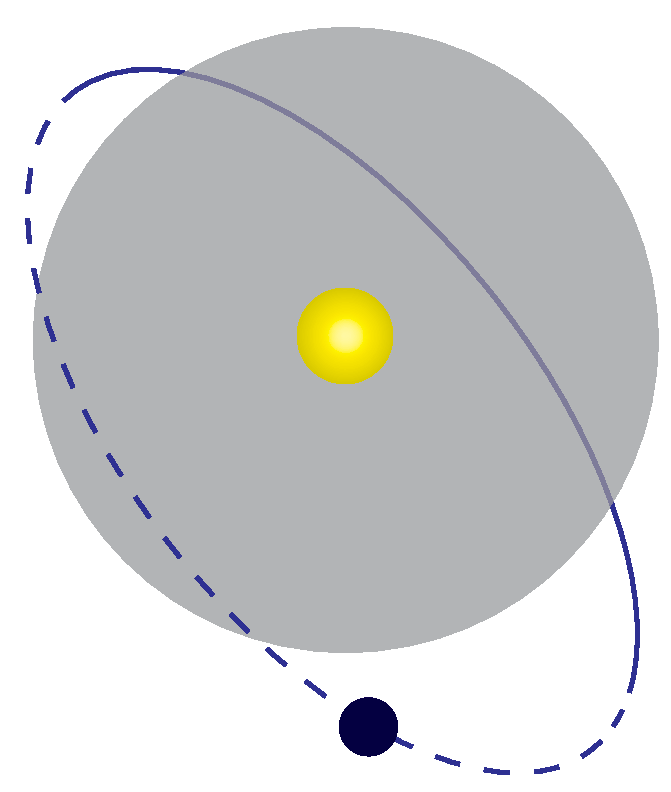
\includegraphics[width=0.3\columnwidth]{imagingConstraintsSchemc}
	\end{center}
	\caption{Schematic of projected exosystem.  Planet is sufficiently illuminated for detection on the solid part of the orbit, and observable outside the gray circle.}
\end{figure}
\vspace{-2ex}
\begin{block}{}
All imaging systems have an inner working angle - the smallest observable separation between star and planet, and a limiting planet brightness.
\end{block}	
}

\subsection*{}
\frame{
\frametitle{Approach}
\begin{enumerate}
\item Define a parameter set suitable for encoding whole exosystems
\item Find mappings between observation methods and parameter set
\item Develop a statistical description of planet observations
\item Develop capability to simulate populations of exosystems 
\item Use these tools to analyze mission concepts and data sets
\end{enumerate}

\begin{itemize}
\item[] D. Savransky and N. ~J.~Kasdin, \emph{Simulation and analysis of sub-$\mu$as precision astrometric data for planet finding}. ApJ 2010.
\item[] D. Savransky,  N.~J.~Kasdin, and E. Cady, \emph{Analyzing the designs of planet finding missions}. PASP 2011.
\item[] D. Savransky,   E. Cady, N.~J.~Kasdin, \emph{Parameter distributions of Keplerian orbits}. ApJ 2011.
\end{itemize}
}

\section{Modeling and Simulation}
\frame{\frametitle{Outline}\tableofcontents[currentsection]}

\subsection{Describing Planets and Orbits}

\frame{
\frametitle{Locating Stars in the Sky}
\framesubtitle{\cite{savransky2010simulation}}
\vspace{-2ex}
\begin{figure}[ht]
 \begin{center}
    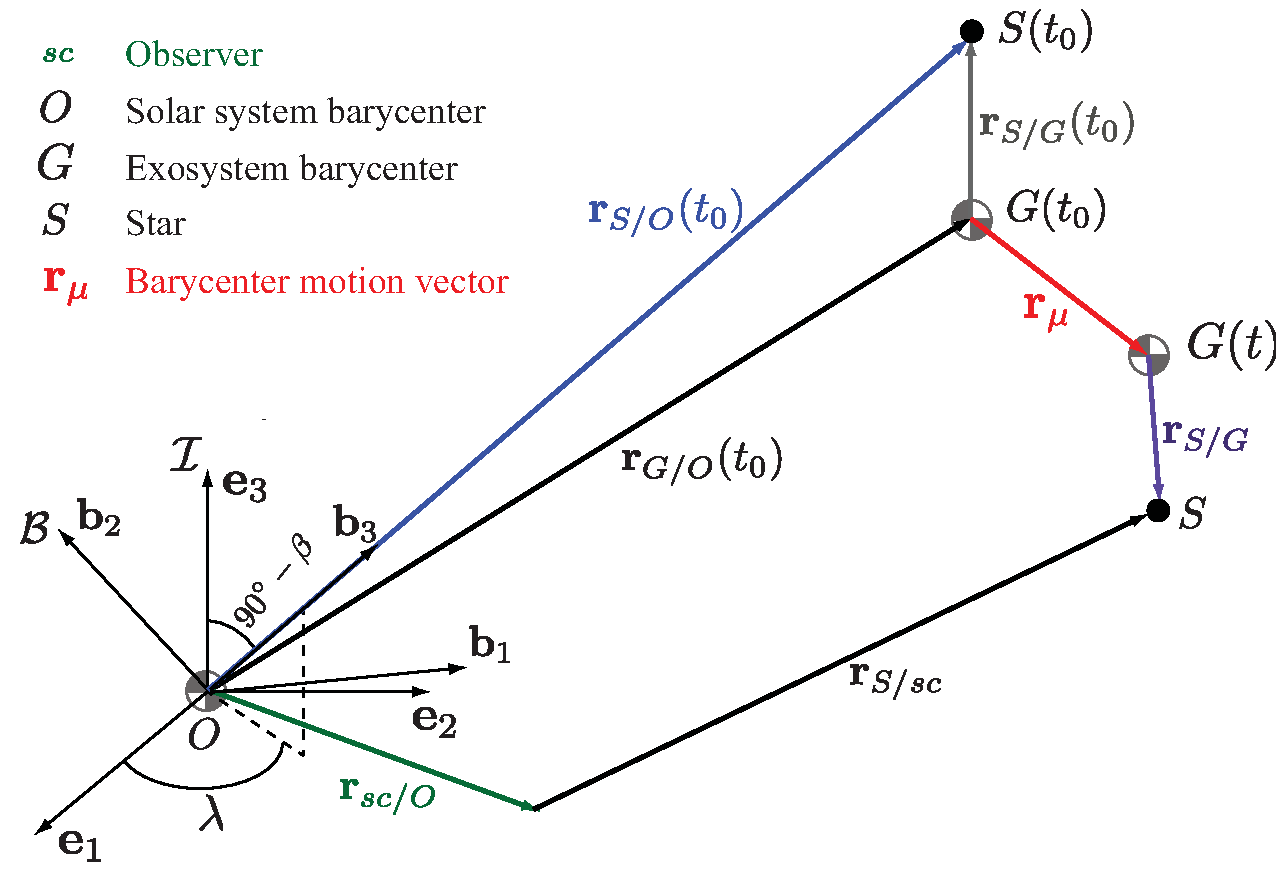
\includegraphics[width=0.85\columnwidth]{ast_model}
 \end{center}
\end{figure}
\vspace{-4ex}
\[
\R_{S/sc} = {\color{MyBlue}\R_{S/O}(t_0)} +  {\color{MyRed}\R_\mu} - {\color{MyGraphite}\R_{S/G}(t_0)} +  {\color{MyPurple}\R_{S/G}} - {\color{MyGreen}\R_{sc/O}}
\]
}


\frame{
\frametitle{System Orientation and Dynamics}
\begin{columns}[c]
\column{0.5\columnwidth}
\vspace{-2ex}
\begin{figure}[ht]
 \begin{center}
    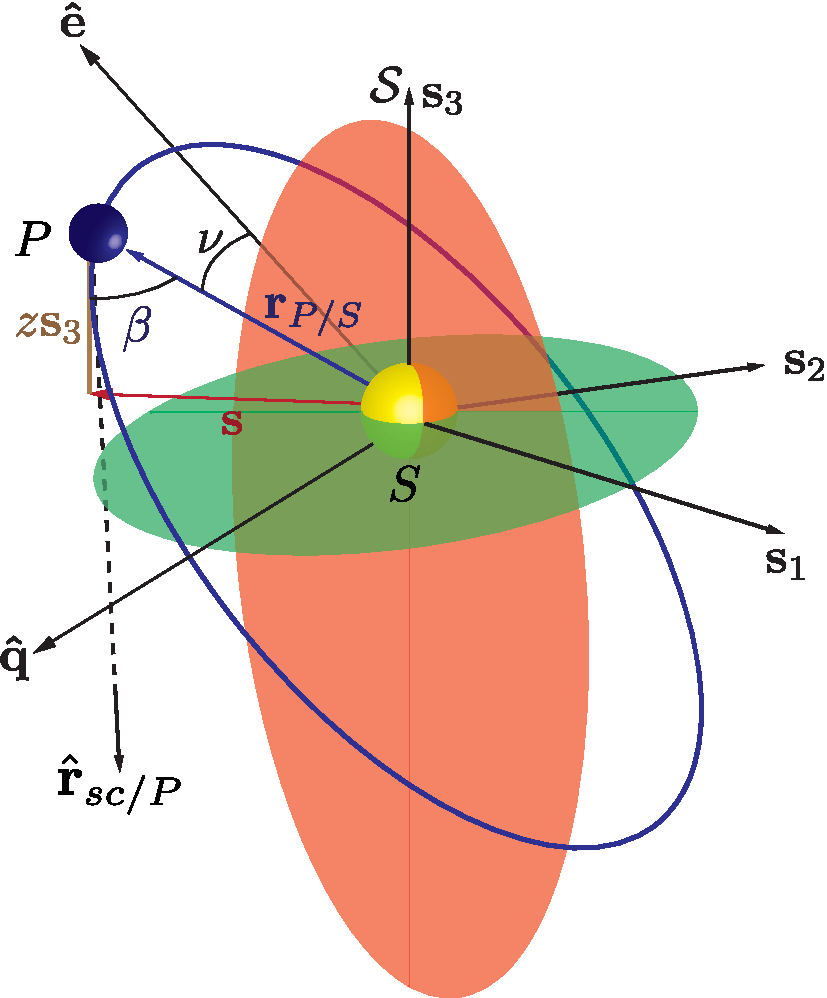
\includegraphics[width=0.9\columnwidth]{orbit_diagram}
 \end{center}
\end{figure}
\vspace{-2ex}
\begin{tabular}{l l l l}
$a$ & Semi-major axis & $\nu$ & True anomaly\\
$e$ & Eccentricity &$\bf s$ & Projected separation
\end{tabular}

\column{0.5\columnwidth}
\[\mf r_{P/S} = r\left(\cos\nu \hat{\mf e} + \sin\nu \hat{\mf q}\right) \]
\[r \triangleq \Vert \mathbf{r}_{P/S} \Vert= \frac{a(1-e^2)}{e \cos(\nu) + 1} \]
\vspace{-4ex}\begin{center}=Orbital radius\end{center}
\begin{align*}
{}^\mc I \mf v_{P/S} =& \sqrt{\frac{\mu_P + \mu_S}{\ell}} \times \\
&\left( -\sin\nu \hat{\mf e} + (e + \cos\nu) \hat{\mf q}\right)
\end{align*}
\[\fdddt{I}{\mf r_{P/S}} + (\mu_S + \mu_P) \frac{\mf r_{P/S}}{\Vert\mf r_{P/S}\Vert^3} = 0 \]

\[ \beta \approx \cos^{-1}\left(\frac{z}{r}\right) \, = \textrm{Phase angle}\]
\end{columns}
}

\frame{
\frametitle{Light From Planets}
\framesubtitle{\cite{brown2005,barman2001irradiated}}
\vspace{-4ex}
\begin{columns}[T]
\column{0.4\columnwidth}
\begin{figure}
	\begin{center}
	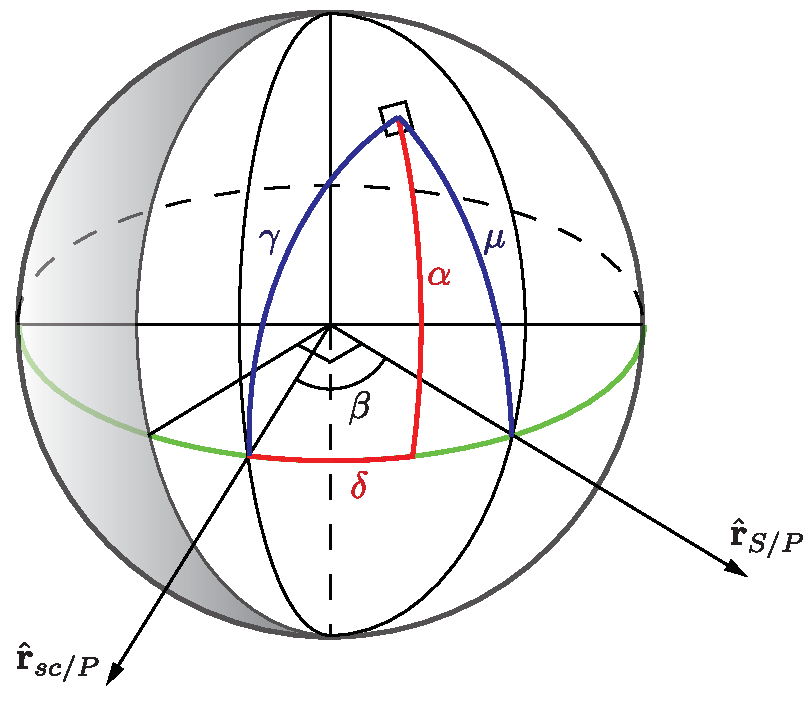
\includegraphics[width=4cm]{../figures/reflection_diagram}
	\caption{Reflecting spherical body \cite{sobolev}}
	\end{center}
\end{figure}
\vspace{-4ex}
\begin{itemize}
\item Flux Ratio:
\[\frac{F^{\textrm{ref}}_P}{F_S} = p \left(\frac{R}{r}\right)^2 \Phi(\beta) \]
\[\Phi_l = \frac{\sin(\beta)+(\pi-\beta)\cos(\beta)}{\pi}\]
\end{itemize}

\column{0.55\columnwidth}
\begin{figure}
	\begin{center}
	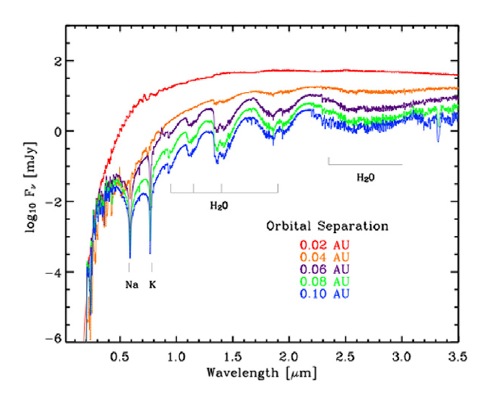
\includegraphics[width=4.5cm]{barman_spectra}
	\vspace{-1ex}
	\caption{Irradiated planet model spectra \cite{hauschildt2008irradiated}}
	\end{center}
\end{figure}
\vspace{-4ex}
\begin{itemize}
\item Day side equilibrium tempearture:
\[\sigma T^4_{\textrm{eq}} = \sigma T^4_{\textrm{int}} + (1 - A)\left(\frac{R}{r}\right)^2F_S\]
where  $L_P = 4\pi R^2 \sigma T^4_{\textrm{int}} $
\end{itemize}
\end{columns}
}

\subsection{Constructing Exosystems}

\frame{
\frametitle{The Parameter Set}
\begin{itemize}
\item Dynamics of exosystem with $n$ planets can be encoded with the state:
\[
X_D = \begin{bmatrix}\R_{P_1/G} & \Rd_{P_1/G} & m_1 & \ldots & \R_{P_n/G} & \Rd_{P_n/G} & m_n & \R_{S/G} & \Rd_{S/G} & m_S \end{bmatrix}^T
\]
where $\Rd \equiv \fddt{I} \R$.
\item Augment state with astrometric and physical constants:
\[
X_C =  \begin{bmatrix} \Rd_\mu & \varpi & \left\{R_i\right\}_1^n  & \left\{p_i\right\}_1^n & R_S &  \left\{T^{\textrm{eff}_i}\right\}_1^n \end{bmatrix}^T
\]
\[ X = \begin{bmatrix} X_D \\ X_C \end{bmatrix} \]
\item Treat observer position $\R_{sc}$ as known
\item May be possible to simplify (or constrain) parameter set by modeling dependencies between mass, radius, age and temperature \cite{fortney2007,sudarsky2005phase}
\end{itemize}
}

\frame{
\frametitle{Exosystem Generation}
\begin{block}{}
How do you simulate populations of exosystems?
\end{block}
\begin{enumerate}
\item Planetary population of interest (i.e., `Earth-like' planets)  - set values or ranges for all orbital and physical planetary parameters
\begin{itemize}
\item Good for studying missions/surveys with specific goals, or doing mission comparisons/trade studies
\end{itemize}
\item Solar system analogue - exosystems composed of  subset of solar system bodies in the solar system
\begin{itemize}
\item Fast way of evaluating effects of multi-planet systems
\end{itemize}
\item Model actual distribution of physical and orbital parameters of known planets based on all available data
\begin{itemize}
\item If trying to closely predict actual results of a survey
\end{itemize}
\item Generate systems starting with simulated nebulae
\begin{itemize}
\item Only needed for testing specific formation theories
\end{itemize}
\end{enumerate}
}

\frame{
\frametitle{Exosystem Orientation}
There are no known biases on exosystem orientation
\begin{columns}[c]
\column{0.5\columnwidth}
\begin{figure}[ht]
 \begin{center}
    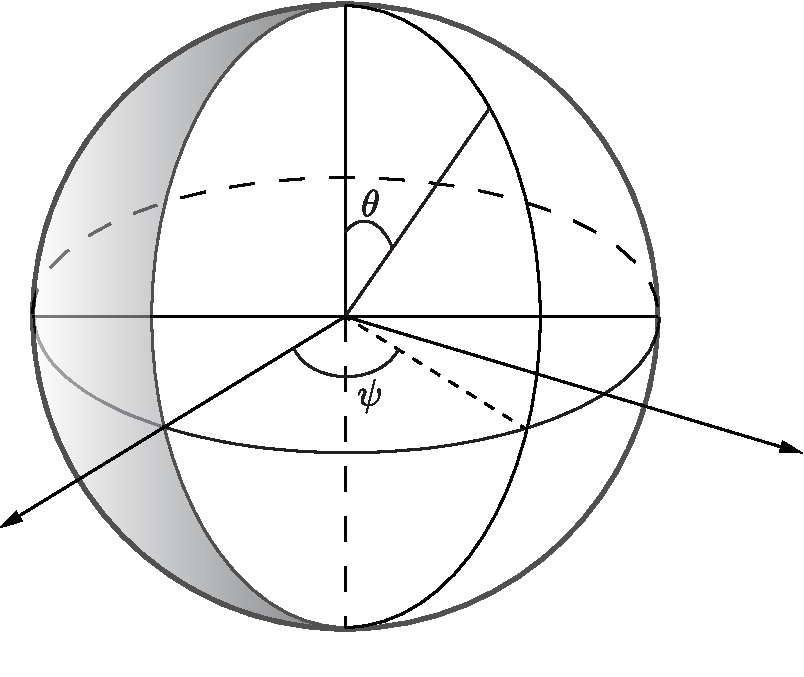
\includegraphics[width=1\columnwidth]{uniformSphere}
 \end{center}
\end{figure}
\column{0.5\columnwidth}
\begin{figure}[ht]
 \begin{center}
    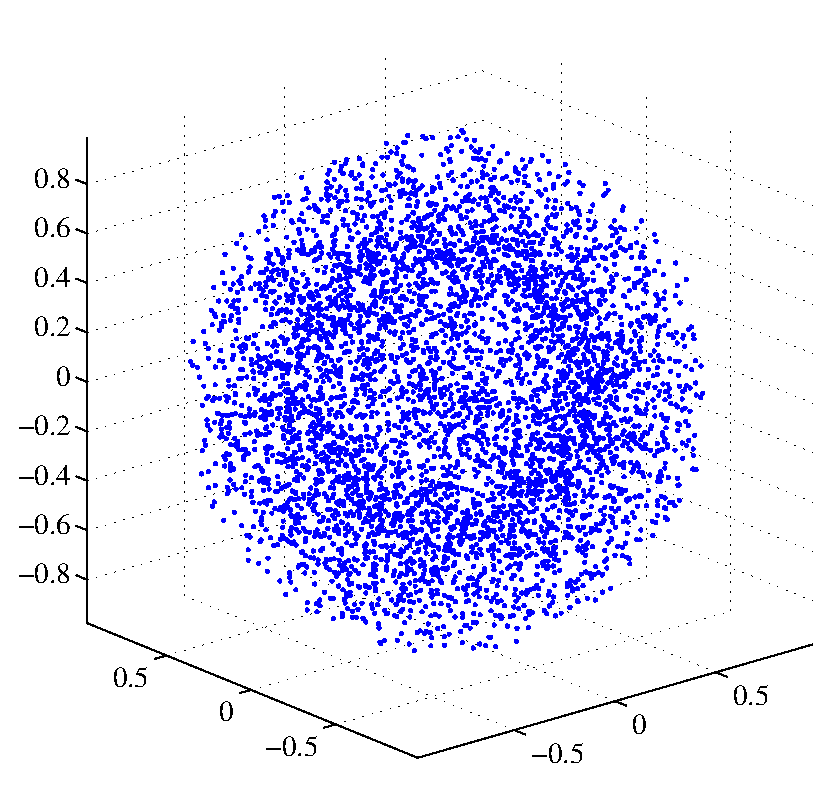
\includegraphics[width=1\columnwidth]{scatterSphere}
 \end{center}
\end{figure}
\end{columns}
\[ \psi \sim U([0,2\pi]) \qquad \theta \sim \cos^{-1}\left( U([-1,1]) \right) \]
}

\frame{
\frametitle{Exosystem Propagation}
Once systems are generated, need to be able to propagate planets forward in time
\vspace{-2ex}
\begin{columns}[c]
\column{0.65\columnwidth}
\begin{figure}[ht]
 \center
 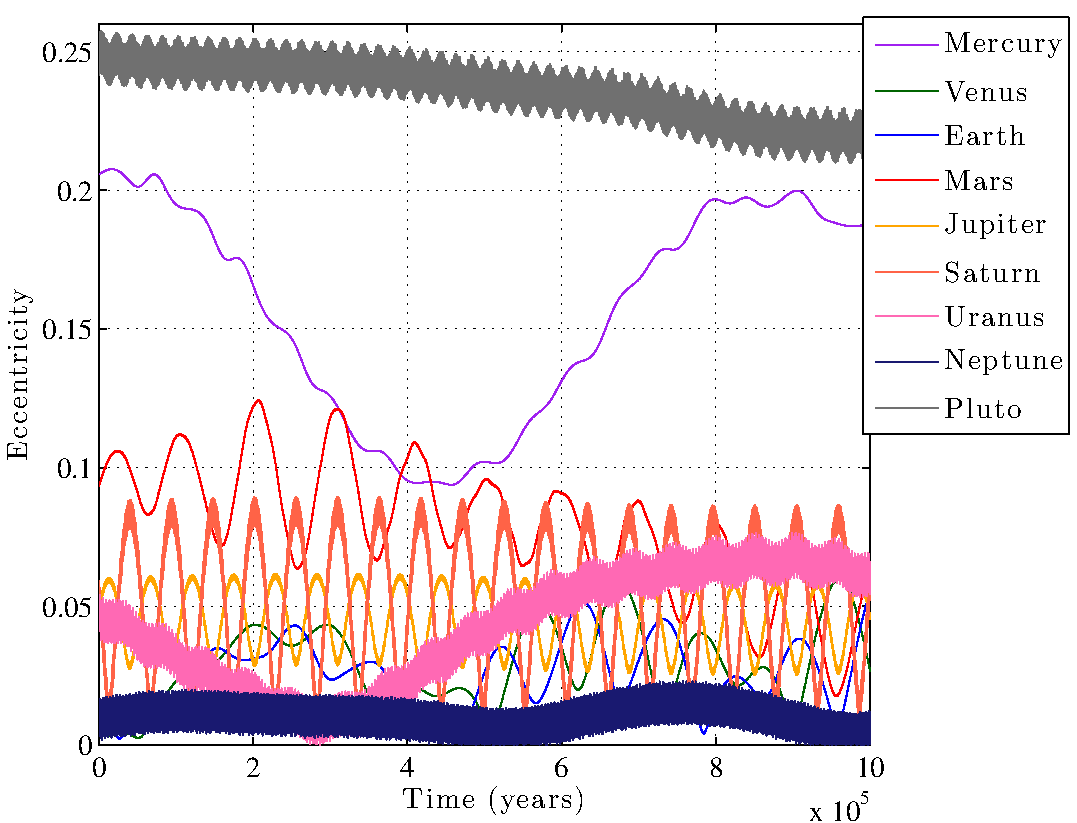
\includegraphics[width = 0.95\columnwidth]{../figures/eccenVar}
  \caption{Variation in orbital eccentricities of solar system bodies over one million years.}
\end{figure}
\column{0.35\columnwidth}
\begin{itemize}
\item Store Keplerian orbital elements, update anomalies (fast but misses n-body effects)
\item Store positions and velocities and integrate (slow but nearly exact)
\item Hybrid scheme \cite{chambers1999hybrid}
\end{itemize}
\end{columns}
}

\frame{
\frametitle{Multi-Planet Stability}
Its highly unlikely that we'll observe unstable systems, so simulated systems should have long-term stability
\begin{figure}[ht]
 \begin{center}
    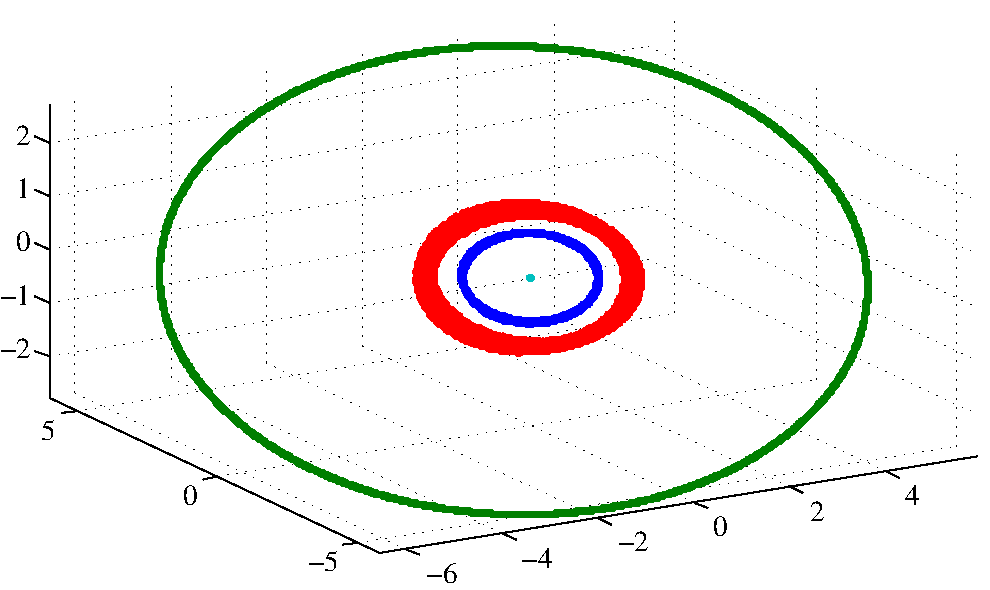
\includegraphics[width=0.75\columnwidth]{../figures/subSolSys}
 \end{center}
 \caption[Sample Multi-body exosystem ]{ Orbits over 1 million years for exosystem composed of analogues of Earth (blue), Mars (red) and Jupiter (green), with a 1.5 $L_\odot$ star.}
\end{figure}
}

\subsection*{}
\frame{
\frametitle{Mapping Instruments to the Parameter Set}
Each observation technique can be described in terms of elements of this parameter set
\begin{itemize}
\item Imaging - planet position and physical parameters
\item Transit photometry - planet and star positions and radii
\item Doppler spectroscopy - star position and velocity
\item Interferometric astrometry - planet and star positions and astrometric parameters
\end{itemize}
\begin{block}{}
We can now describe exosystems and the data produced by observing them with various instruments using one unified parameter set.
\end{block}
}

\section{Applications}

\frame{\frametitle{Outline}\tableofcontents[currentsection]}

\subsection{Detection Statistics}

\frame{
\frametitle{Direct Detection Observable Distribution}
\framesubtitle{\cite{brown2005}}
\vspace{-2ex}
\only<1>{
\begin{figure}[ht]
\centering
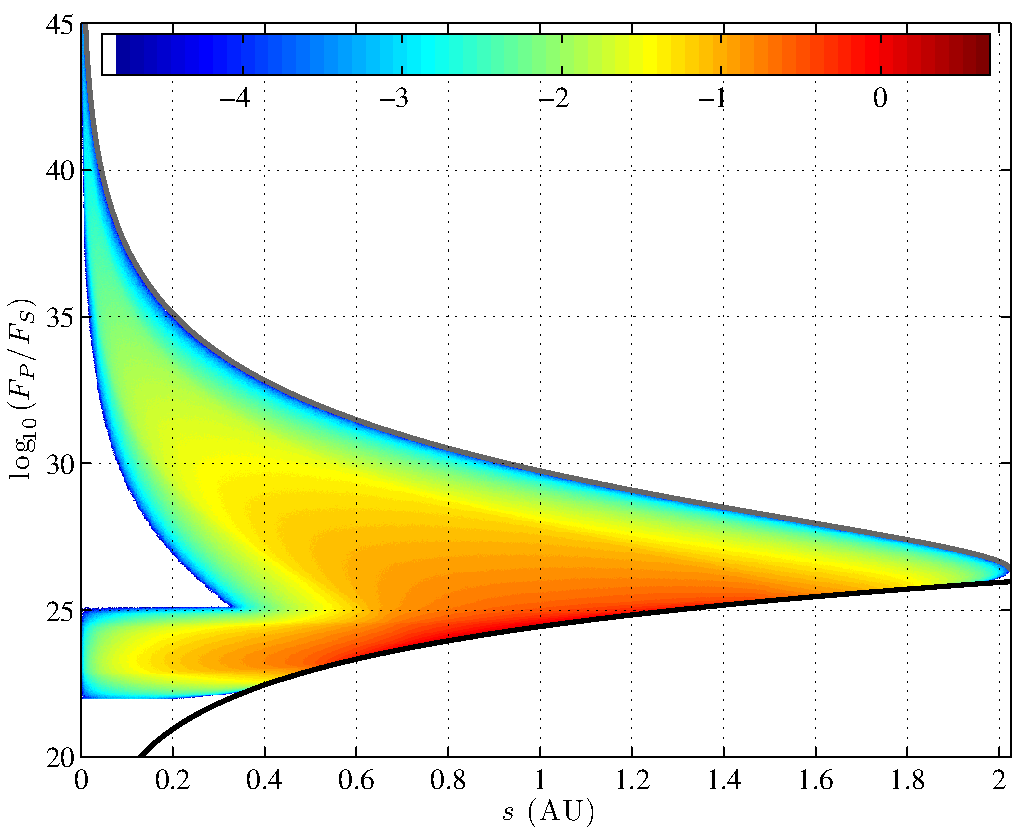
\includegraphics[width=0.65\textwidth]{../figures/earthTwin_pdf}
\vspace{-2ex}
 \caption[Earth-twin observation PDF]{ Joint probability density function of ($\bar s = s,\bar F_P/F_S = F_P/F_S$) for Earth-twin planets ($a \in [0.7, 1.5]$, $e \in [0, 0.35]$, $p = p_\oplus$, $R = R_\oplus$) sampled via 1 billion Monte Carlo trials.}
\end{figure} 
}
\only<2>{
\begin{figure}[ht]
\centering
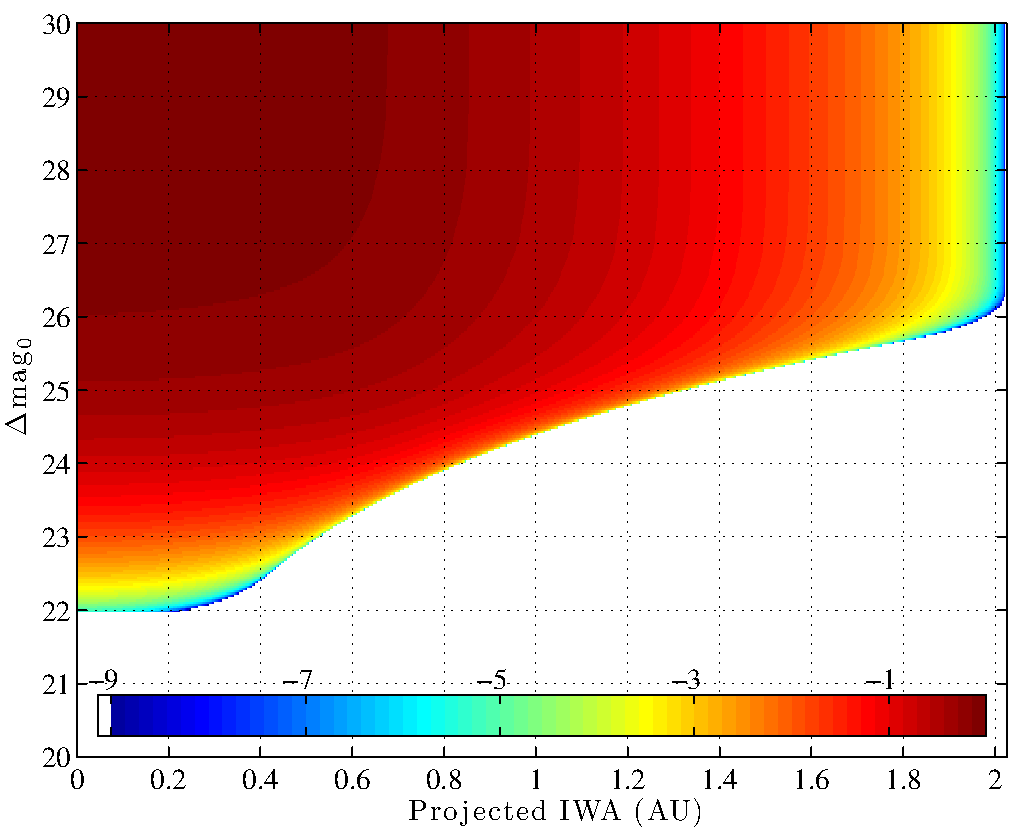
\includegraphics[width=0.65\textwidth]{../figures/earthTwin_cdf}
\vspace{-2ex}
 \caption[Earth-twin observation PDF]{ Joint cumulative distribution function of ($\bar s = s,\bar F_P/F_S = F_P/F_S$) for Earth-twin planets ($a \in [0.7, 1.5]$, $e \in [0, 0.35]$, $p = p_\oplus$, $R = R_\oplus$) sampled via 1 billion Monte Carlo trials.}
\end{figure} 
}
}

\frame{
\frametitle{Monte Carlo is Inefficient}
\vspace{-2ex}
\only<1>{
\begin{figure}[ht]
\centering
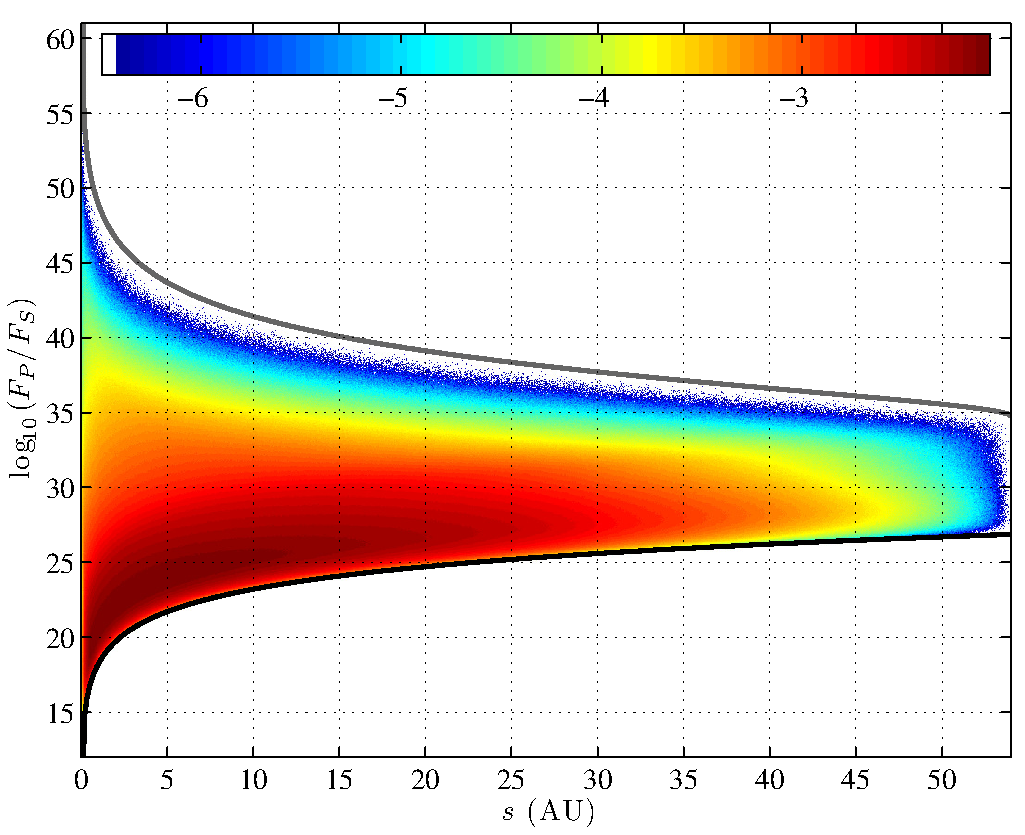
\includegraphics[width=0.65\textwidth]{../figures/undersampled_comp_pdf}
\vspace{-2ex}
 \caption[Earth-twin observation PDF]{ Joint probability density function of ($\bar s = s,\bar F_P/F_S = F_P/F_S$) for a randomized planetary population  ($a \in [0.4, 30]$, $e \in [0, 0.8]$, $p \in [0.1, 0.5]$, $R \in [0.7, 11.2]R_\oplus$) sampled via 1 billion Monte Carlo trials.}
\end{figure} 
}
\only<2>{
\begin{figure}
	\begin{center}
	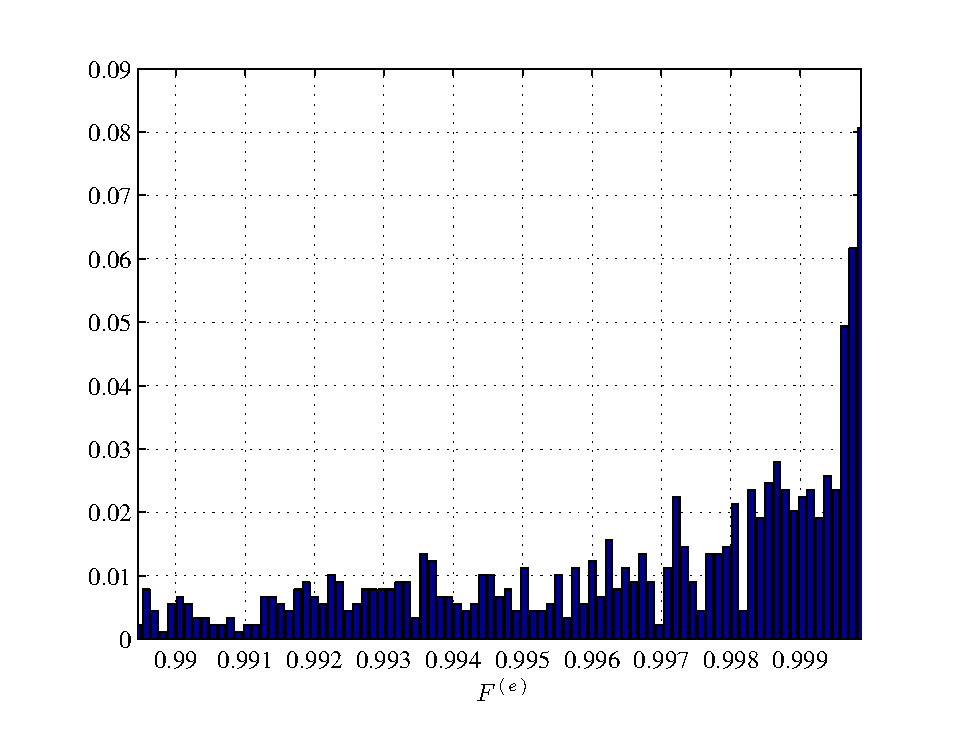
\includegraphics[width=0.75\columnwidth]{photHist}
	\caption[]{ Probability density function for transit flux ratio ($\bar F^{(e)} = F^{(e)}$).}
	\end{center}
\end{figure}
}
}

\frame{
\frametitle{Distributions of Keplerian Orbital Elements}
\framesubtitle{\cite{savransky2011parameter}}
If you know the distribution functions of the observables, you can directly sample the completeness function.  Assume:
\begin{itemize}
\item Exosystem orientations are uniform wrt the observer
\item Distributions for semi-major axis and eccentricity are known
\end{itemize}

\begin{columns}[c]
\column{0.65\columnwidth}
\begin{figure}
	\begin{center}
	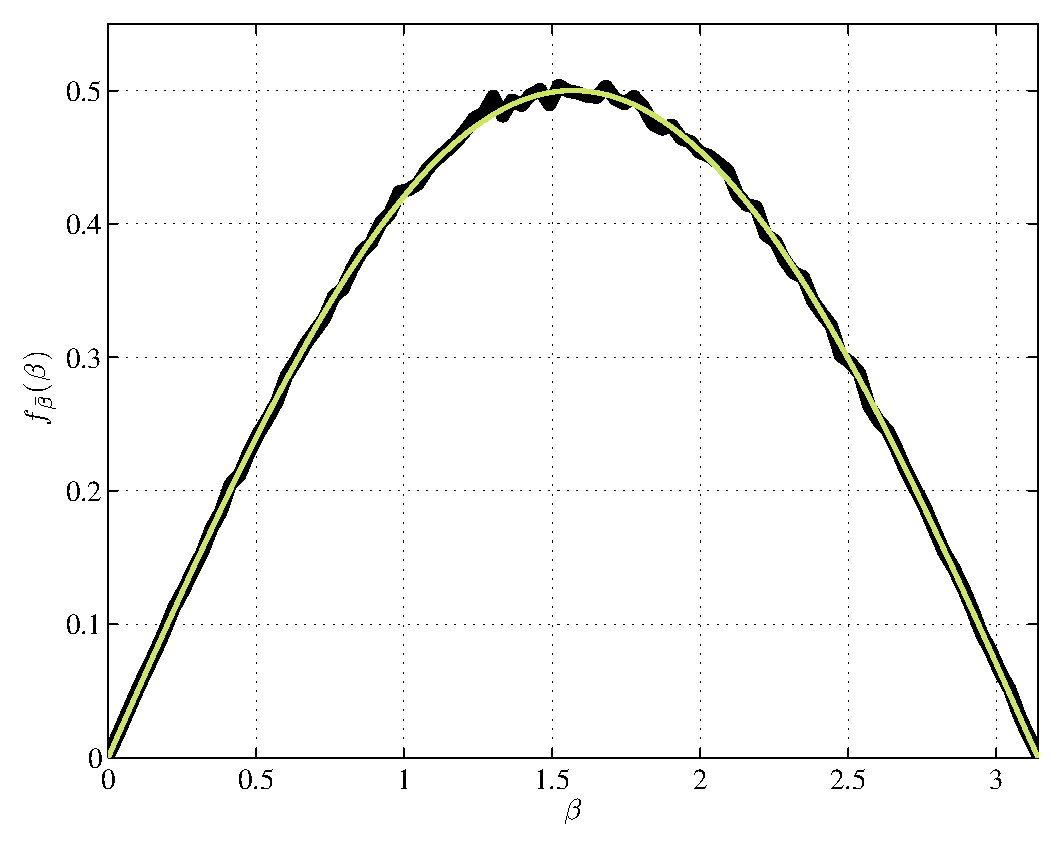
\includegraphics[width=0.725\columnwidth]{../figures/betadist}
	\vspace{-2ex}
	\caption{Phase angle PDF: Monte Carlo (black) and algebraic solution (green)}	
\end{center}
\end{figure}

\column{0.3\columnwidth}
\begin{block}{}
\centering
$\beta$ is always sinusoidally distributed!
\end{block}
\end{columns}
}

\frame{
\frametitle{Direct Sampling vs. Monte Carlo}
\only<1>{
\begin{figure}
	\begin{center}
	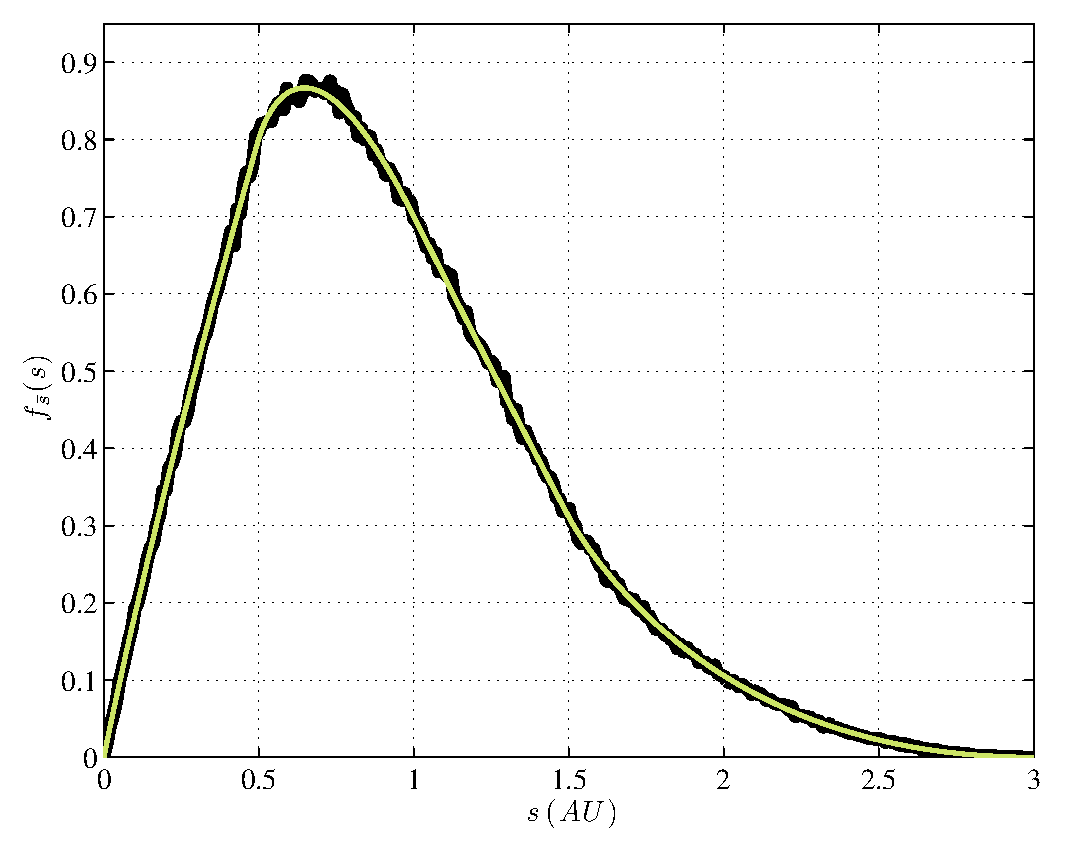
\includegraphics[width=0.7\columnwidth]{../figures/sint}
	\vspace{-2ex}
	\caption{Probability density function of apparent separation using Monte Carlo (black) and algebraic solution (green) for uniform $a$ and $e$.}	
\end{center}
\end{figure}
}
\only<2>{
\begin{figure}[ht]
\centering
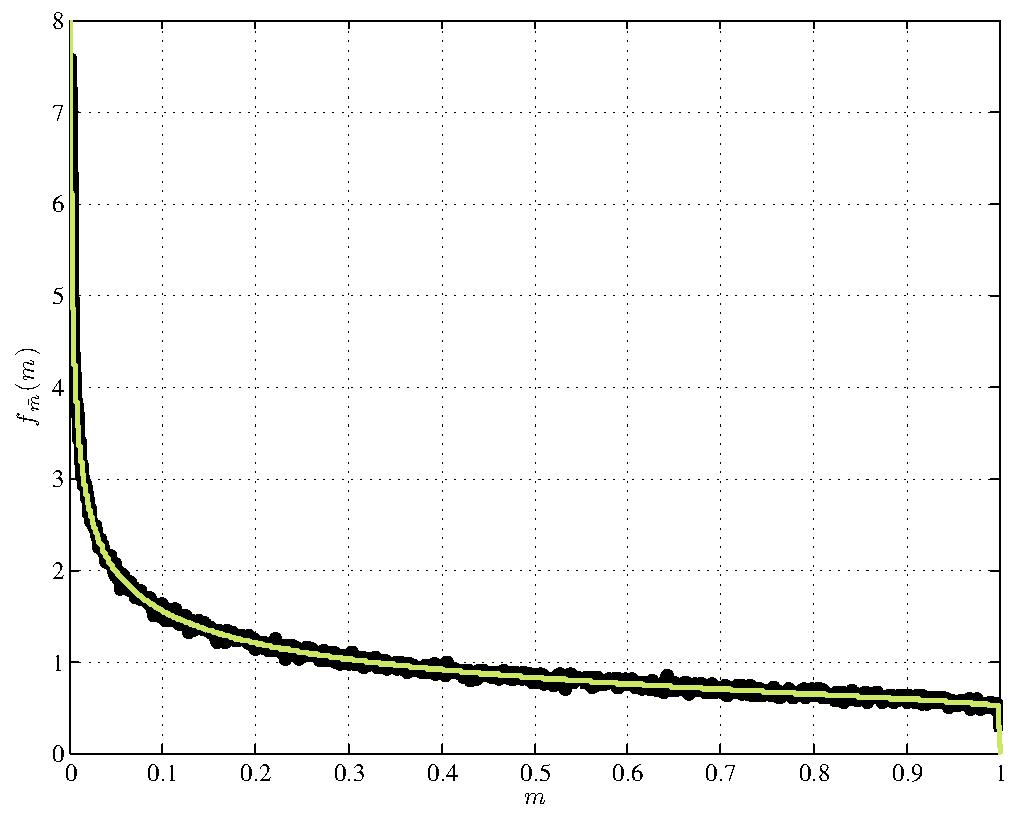
\includegraphics[width=0.7\columnwidth]{../figures/mdist}
\vspace{-2ex}
\caption{Probability density function of Lambert phase function $m = \Phi(\beta)$ using Monte Carlo (black) and algebraic solution (green).}
\end{figure} 
}
}

\frame{
\frametitle{Period Estimation}
\vspace{-2ex}
\[ P_{orb} = 2\pi\sqrt{a^3/(\mu_S + \mu_P)} \]
\begin{itemize}
\item Assume $\mu_S >> \mu_P$ and get $\mu_S$ from mass-luminosity relationship \cite{henry1993}
\item Need to estimate the semi-major axis
\end{itemize} 
\[ f_{\bar s\vert\bar a}\left(s \vert a\right)  = \frac{1}{\pi}  \int_{0}^1  \int_{0}^{1} \frac{s}{a\sqrt{\left(1 - l^2\right)\left[(ael)^2 - (al-s)^2\right]}}f_{\bar{e}}(e) \, \mathrm{d}e \, \mathrm{d}l  \]
\[\hat a = \arg\max_{a \in \bar a}   \frac{1}{\pi}  \int_{0}^1  \int_{0}^{1} \frac{s_0}{a\sqrt{\left(1 - l^2\right)\left[(ael)^2 - (al-s_0)^2\right]}}f_{\bar{e}}(e) \, \mathrm{d}e \, \mathrm{d}l \]
\medskip
\begin{block}{}
\[ \hat a = s_0 \]
\end{block}
}

\frame{
\frametitle{Semi-major Axis Estimation}
\vspace{-2ex}
\begin{figure}[ht]
\centering
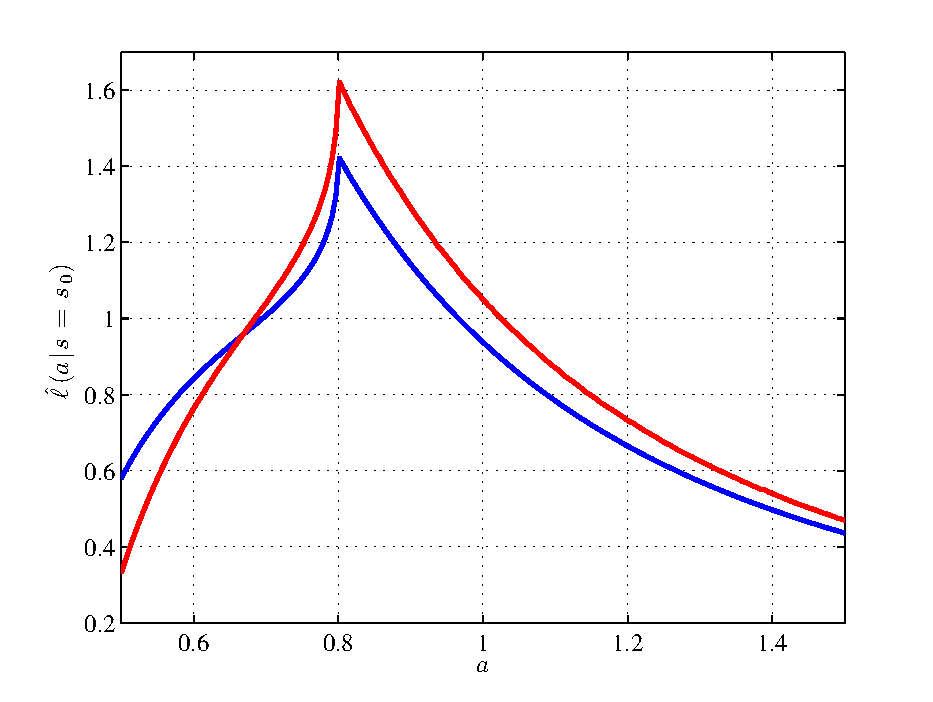
\includegraphics[width=0.75\columnwidth]{../figures/amle}
%add better labels
\vspace{-2ex}
\caption{Likelihood function for semi-major axis given one observation of apparent separation $s_0 = 0.8$ for uniform distribution of $a$ (in AU) and uniformly distributed (red) or step-distributed $e$ (blue). }
\end{figure} 
}

\subsection{Mission Analysis}

\frame{
\frametitle{Mission Simulation}
\framesubtitle{\cite{savransky2010}}
\begin{itemize}
	\item Create descriptions of instruments, planetary orbits/properties and observations
	\item Generate ensembles of full mission simulations (timelines of observations)
	\item Extract distributions of science yield/performance metrics
\end{itemize}

\begin{figure}[ht]
\centering
   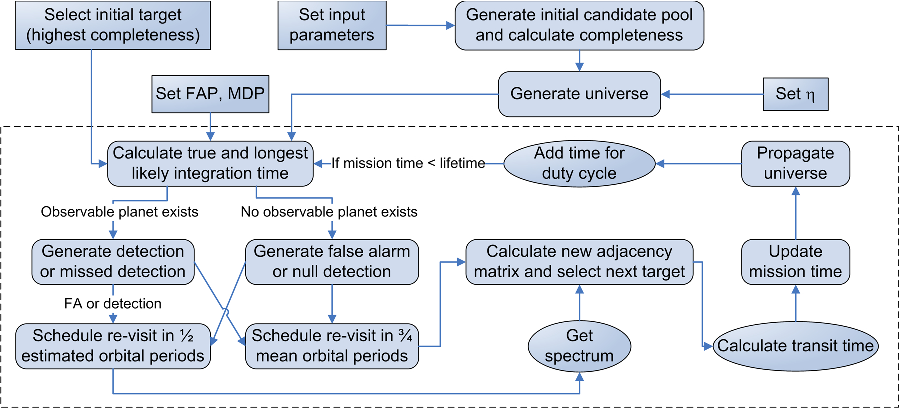
\includegraphics[width = 0.75\columnwidth]{../figures/simFlowchart}
 \caption{Flowchart of simulation framework}
 \end{figure}
}

\frame{
\frametitle{Visits as a Graph}
\begin{columns}
	\column{0.5\columnwidth}
	\begin{figure}
		\begin{center}
		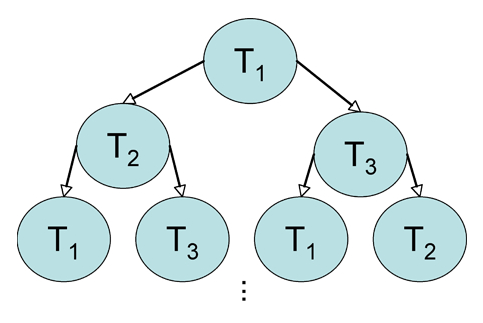
\includegraphics[width=0.8\columnwidth]{visit_graph}
		\caption{Visit graph for 3 target pool.}
		\end{center}
	\end{figure}
	
	\column{0.5\columnwidth}
	\begin{itemize}
		\item Each set of possible transitions on the visit graph can be represented as a weighted adjacency matrix.
		\item The weights of the matrix entries represent the `cost' of choosing the next star. 
	\end{itemize}
\end{columns}
The cost of transitioning from target $i$ to target $j$ is:
\[
\begin{split}
A_{ij}  &= \left[ a_1 \frac{\cos^{-1}\left(u_i \cdot u_j\right)}{2\pi}B_{inst} + a_2 \textrm{comp}_j  - a_3 e^{t_c-t_f} B_{unvis} +  a_4 B_{vis}(1-B_{revis}) \right. \\ 
&\left.{}  - a_5 B_{revis} \left(\frac{N_j}{N_{req}} \right)(N_j < N_{req}) - a_6 \frac{\tau_j}{\textrm{vis}_j} \right] /(1-B_{keepout})
\end{split}
\]
}

\frame{
\frametitle{Local Optimality of Decision Modeling}
\begin{figure}[ht]
 \begin{center}
   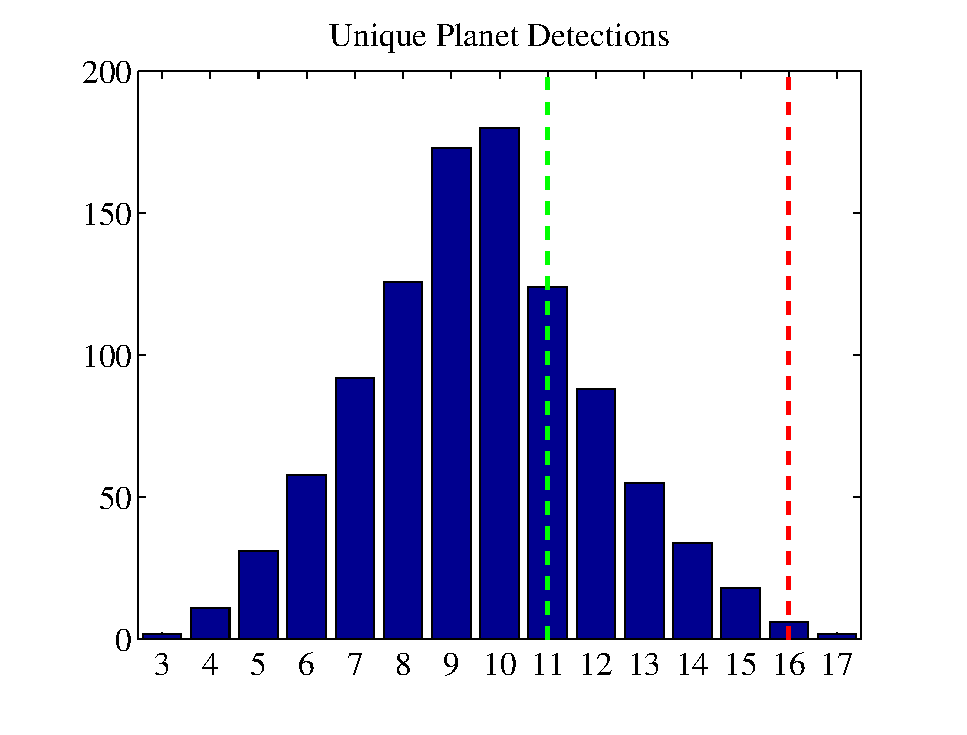
\includegraphics[width=0.45\columnwidth,clip=true,trim=0.4in 0.25in 0.4in 0in]{../figures/optimhistsc} 
   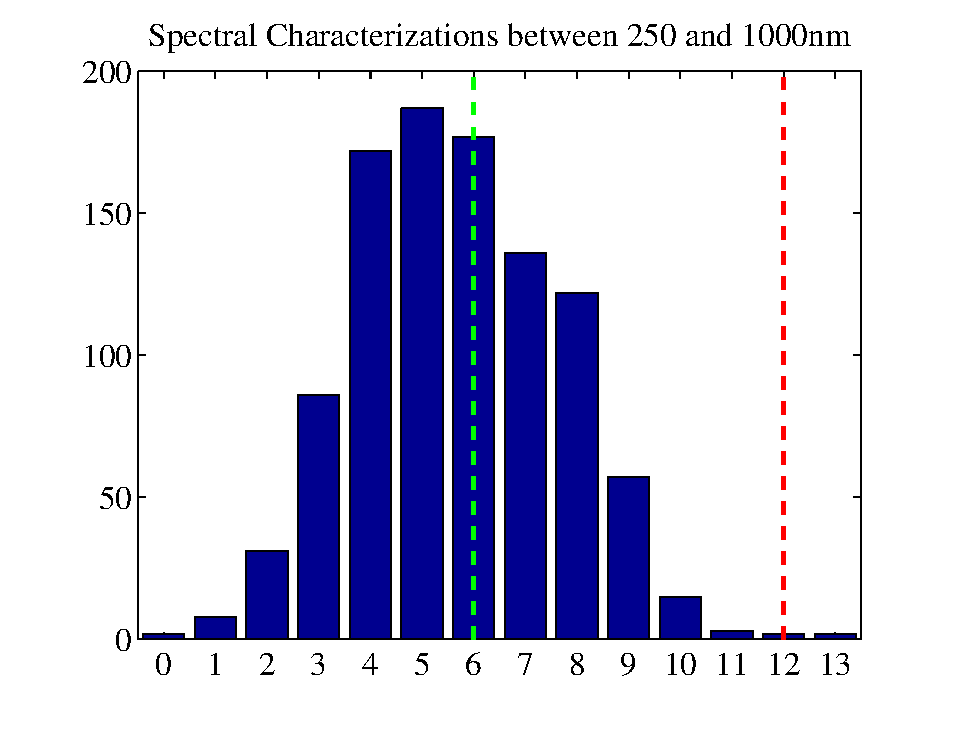
\includegraphics[width=0.45\columnwidth,clip=true,trim=0.4in 0.25in 0.4in 0in]{../figures/optimhistsd}
 \end{center}
 \caption[]{Comparison of scientific yield from automated visit order selection and randomized visit order.  The blue bars are histograms of results from 1000 mission simulations using randomized visit order.  Red dashed lines are results from the automated visit order. Green dashed lines are results obtained by always going to the next highest completeness target.}
 \end{figure}
}

\frame{
\frametitle{Mission Analysis}
\vspace{-2ex}
\only<1>{
\begin{figure}[ht]
 \begin{center}
  \begin{tabular}{c c}
   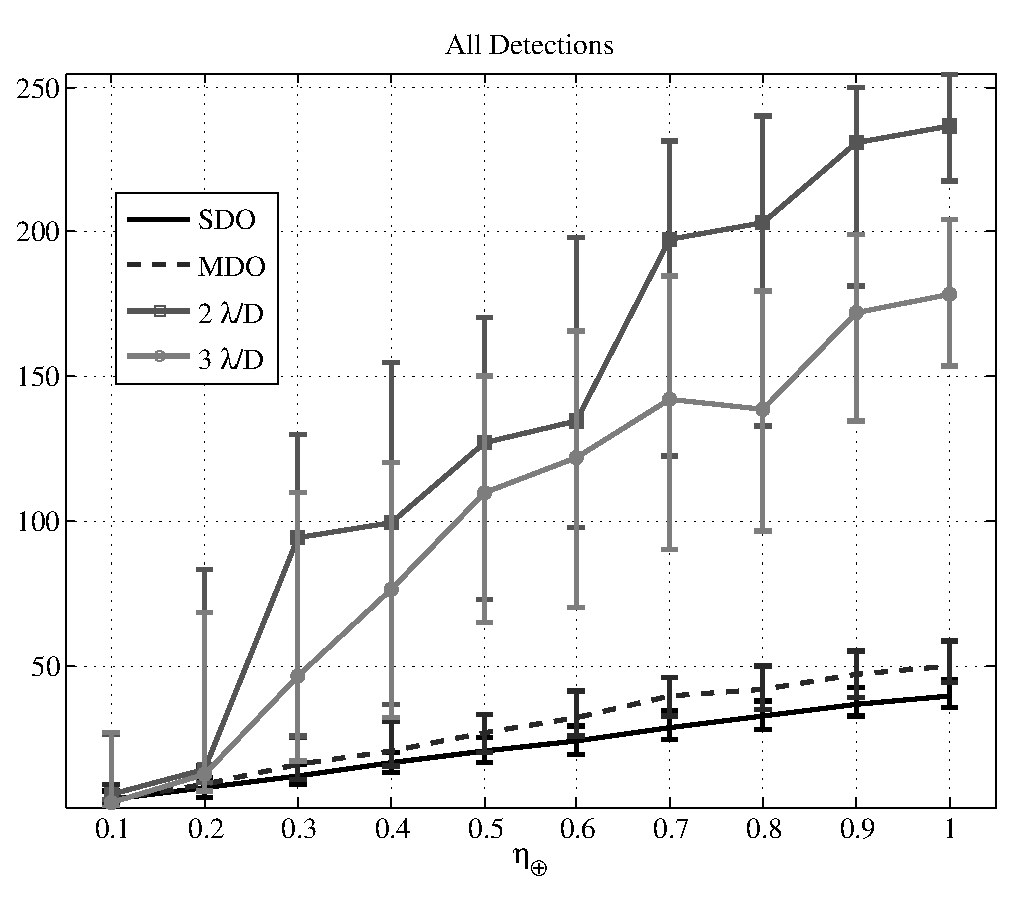
\includegraphics[width=0.35\columnwidth]{../figures/c4m_ADETs} &
   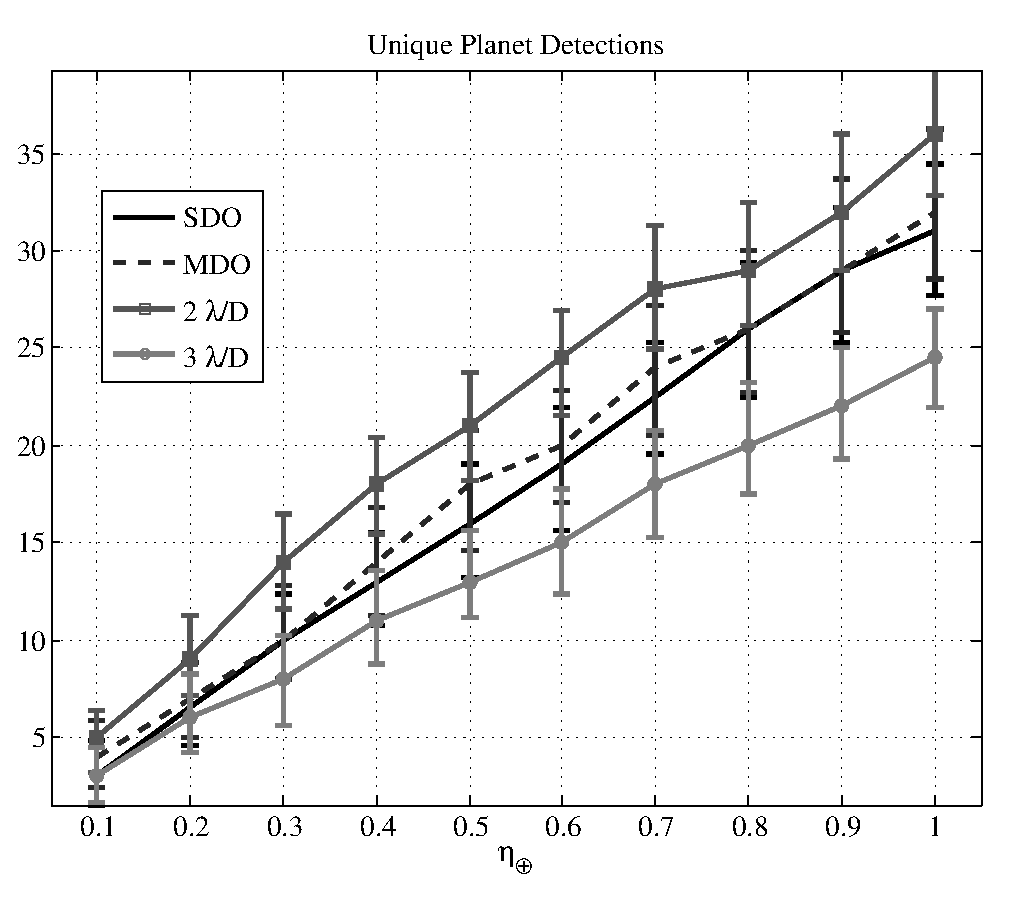
\includegraphics[width=0.35\columnwidth]{../figures/c4m_AuDETs} \\
   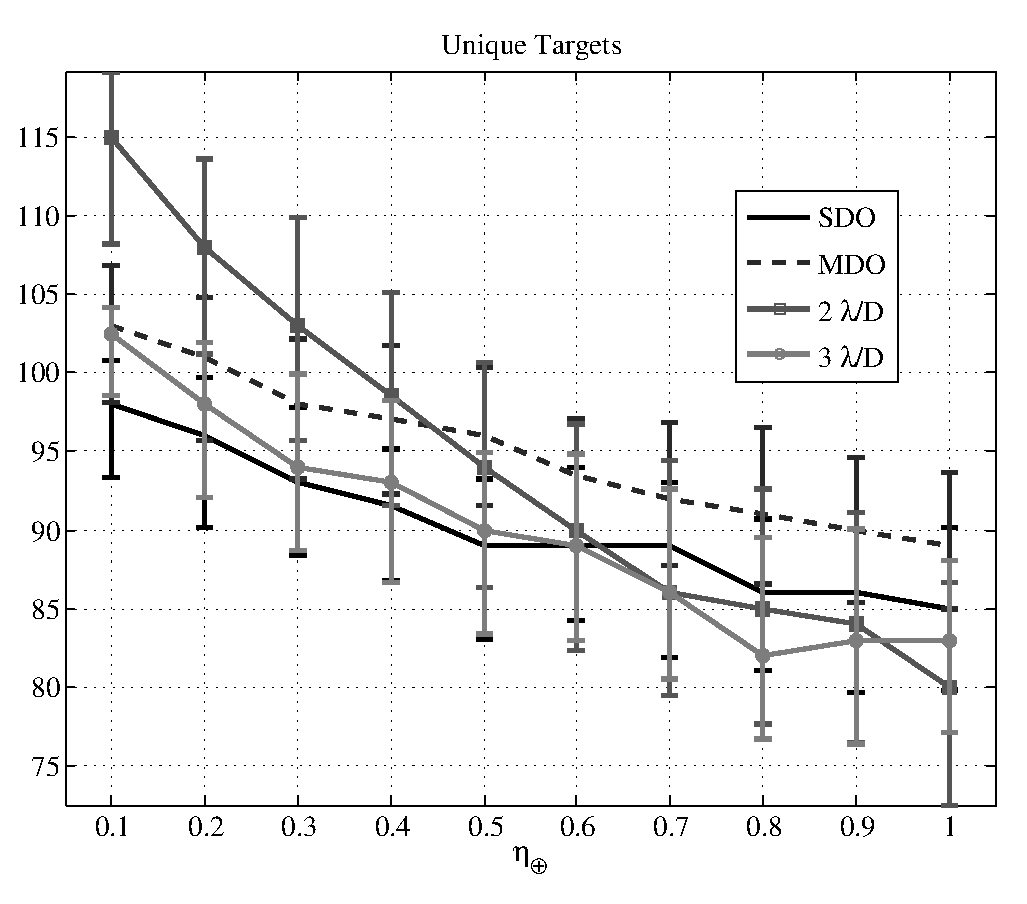
\includegraphics[width=0.35\columnwidth]{../figures/c4m_Auvisits} &
   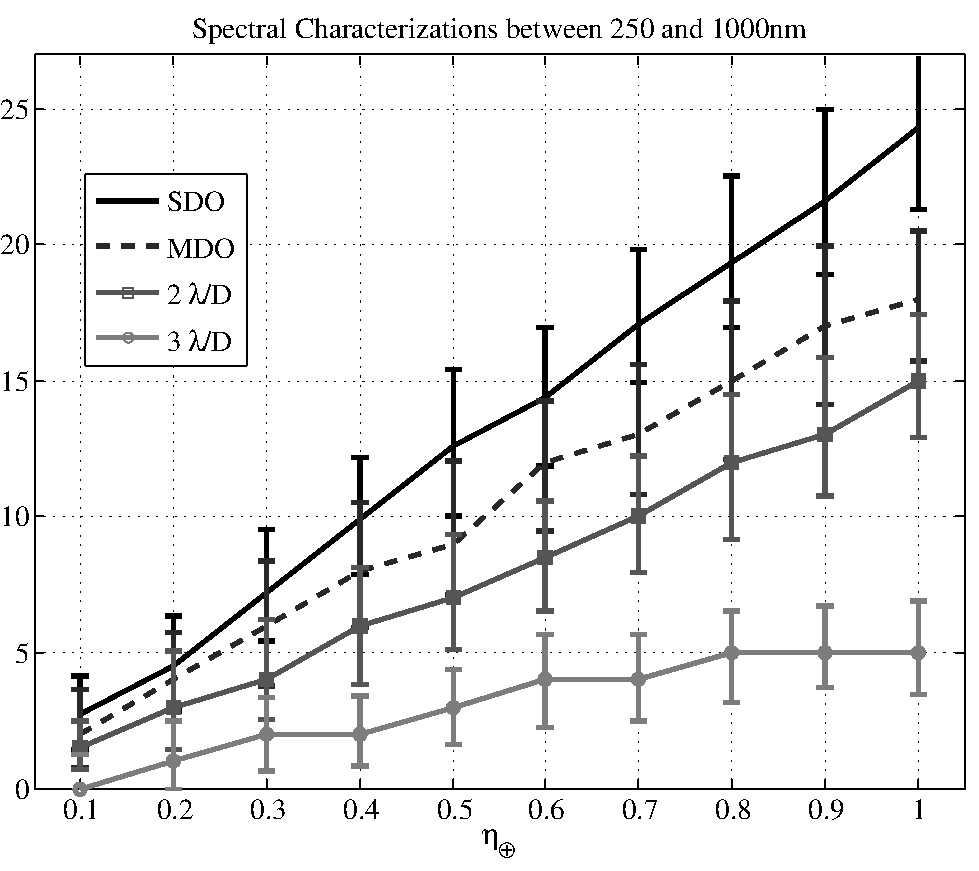
\includegraphics[width=0.35\columnwidth]{../figures/c4m_ASPECTRA}
  \end{tabular}
 \end{center}
 \end{figure}
 \vspace{-3ex}\begin{center} 4 m Telescope \end{center}
}
\only<2>{
\begin{figure}[ht]
 \begin{center}
  \begin{tabular}{c c}
   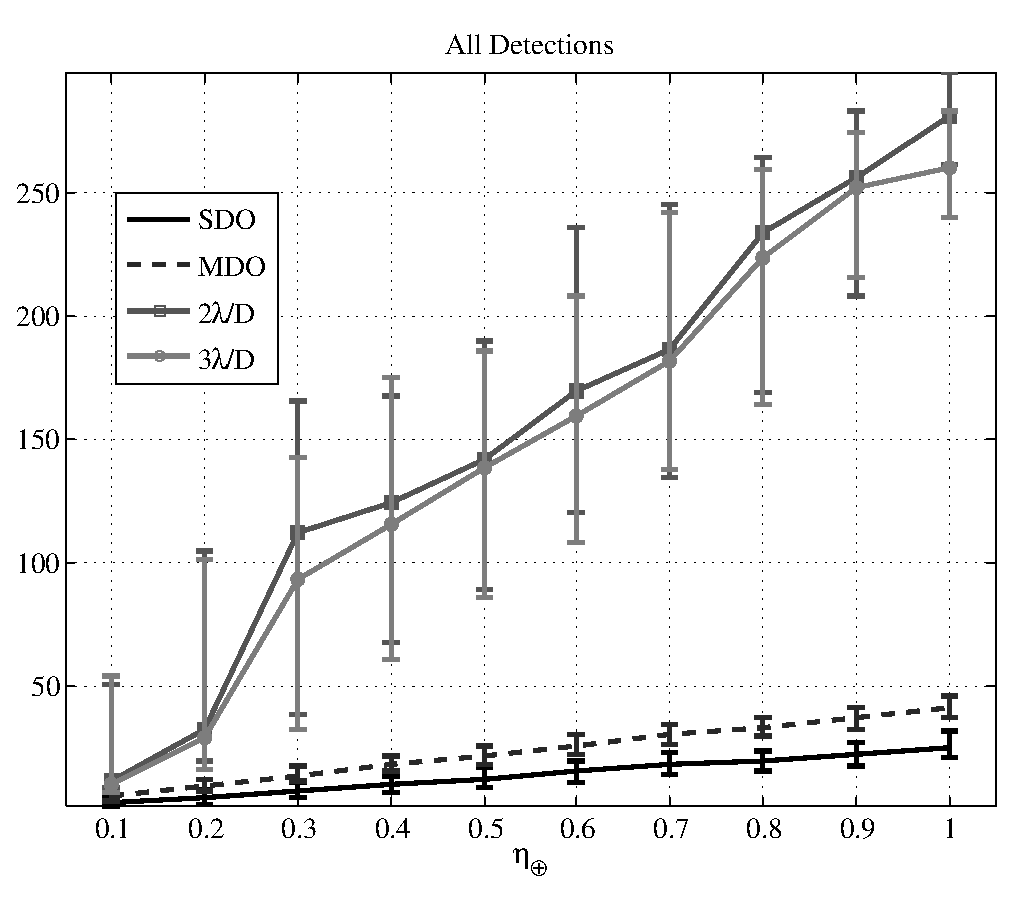
\includegraphics[width=0.35\columnwidth]{../figures/c8m_ADETs} &
   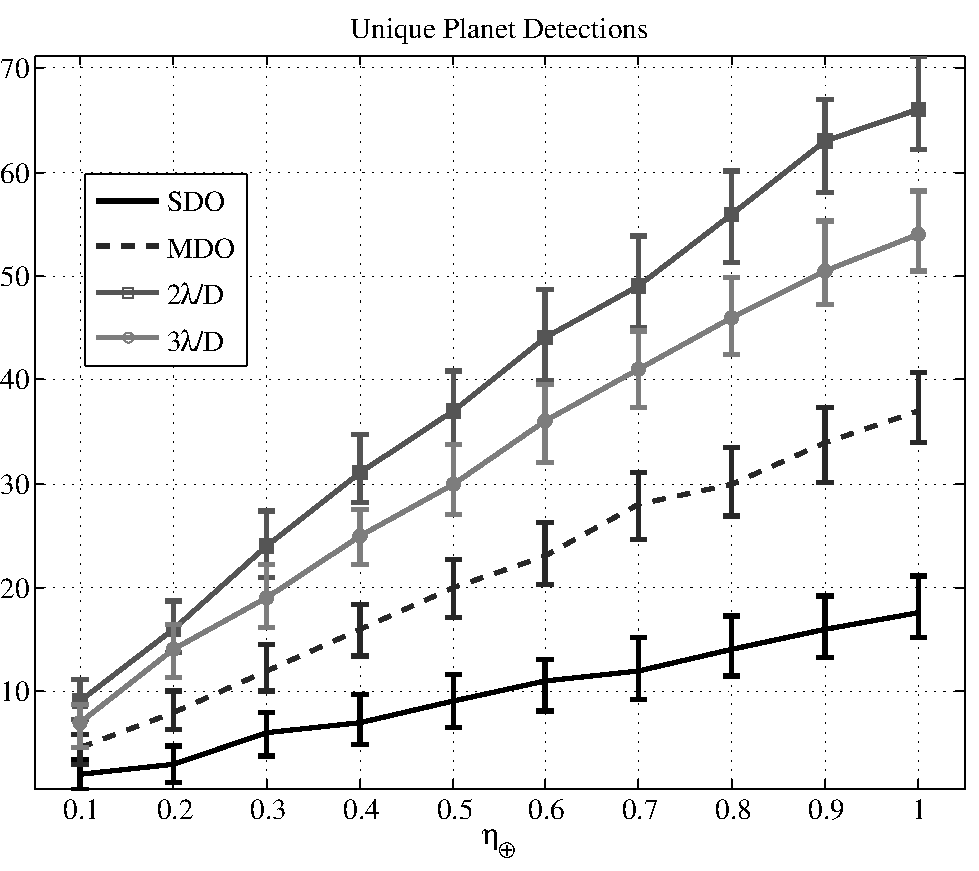
\includegraphics[width=0.35\columnwidth]{../figures/c8m_AuDETs} \\
   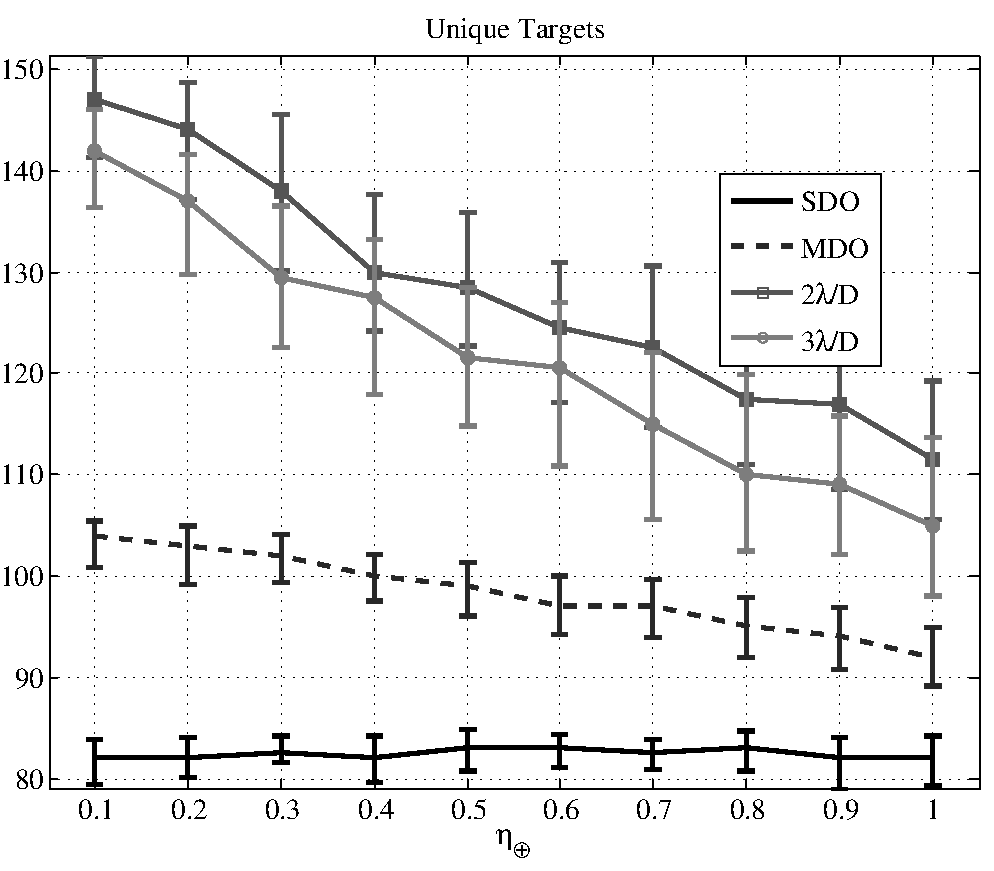
\includegraphics[width=0.35\columnwidth]{../figures/c8m_Auvisits} &
   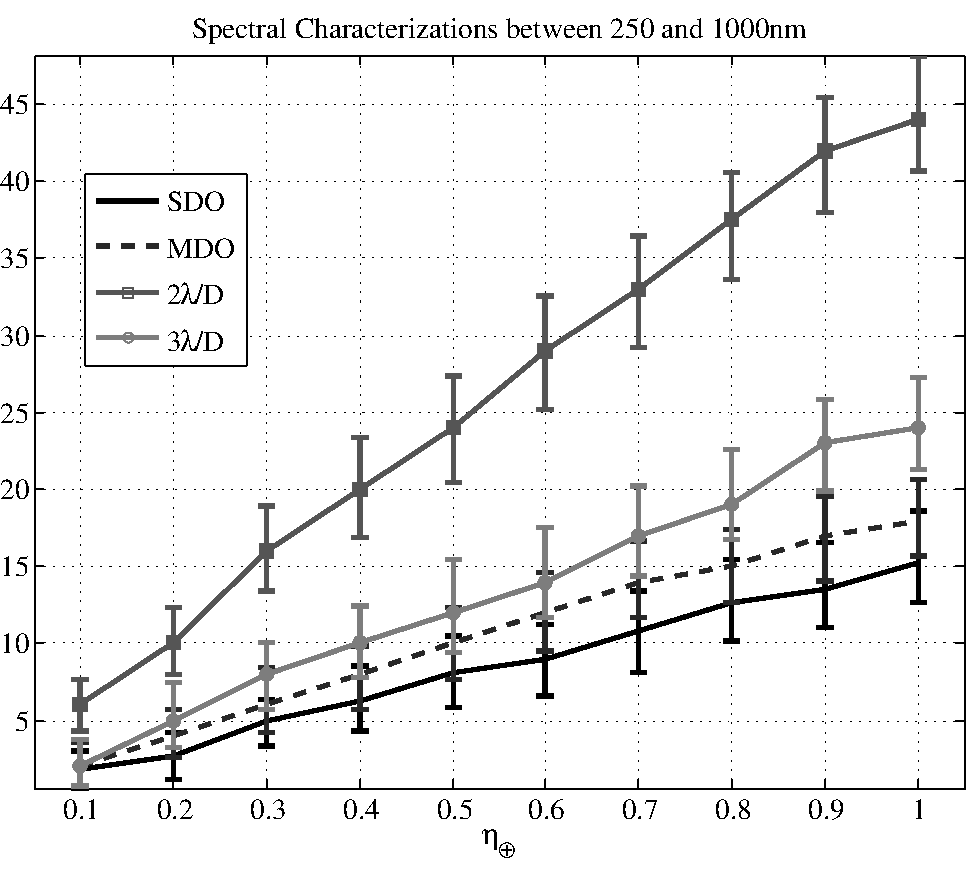
\includegraphics[width=0.35\columnwidth]{../figures/c8m_ASPECTRA}
  \end{tabular}
 \end{center}
 \end{figure}
 \vspace{-3ex}\begin{center} 8 m Telescope \end{center}
}
\only<3>{
 \begin{figure}[ht]
 \begin{center}
  \begin{tabular}{c c}
   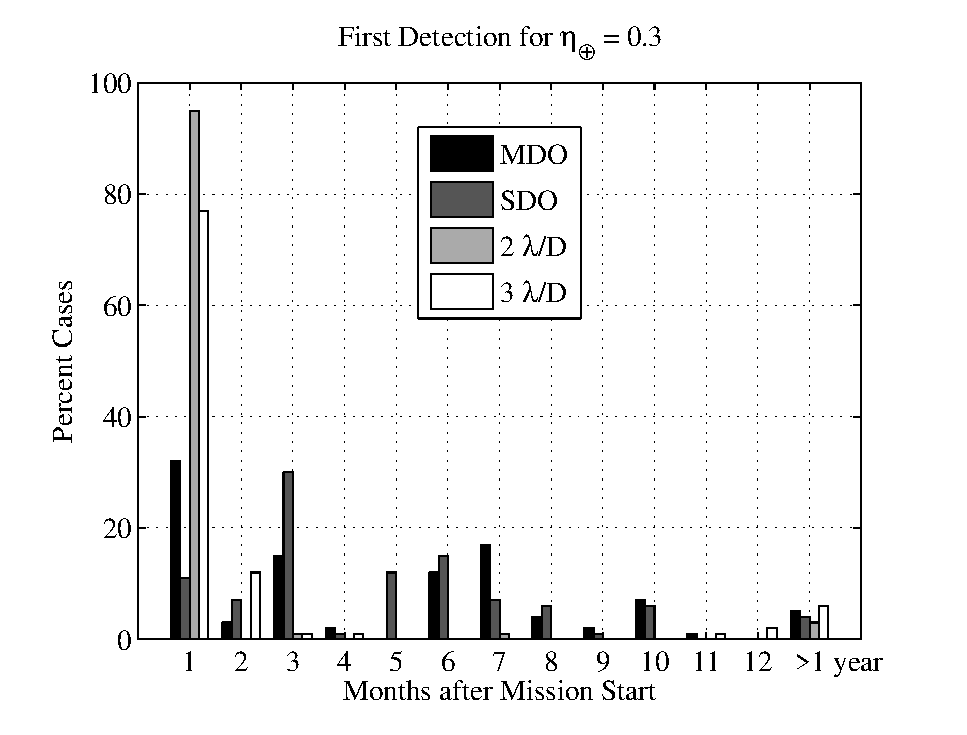
\includegraphics[width=0.48\columnwidth]{../figures/c4_firstDetHist} &
   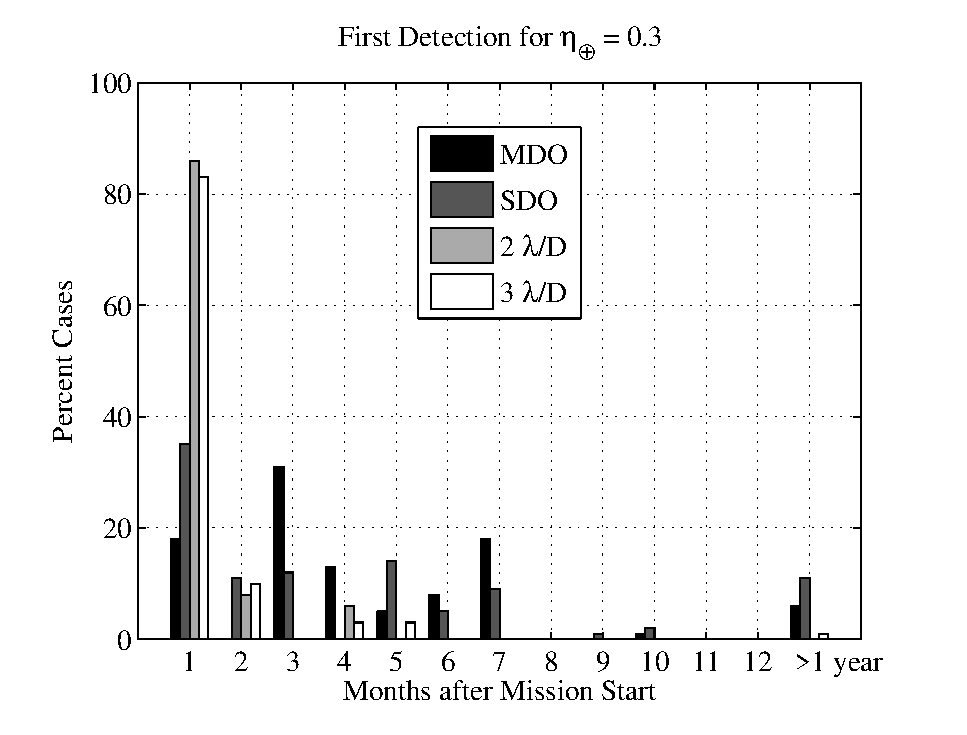
\includegraphics[width=0.48\columnwidth]{../figures/c8_firstDetHist}\\
   4 m Telescope & 8 m Telescope
   \end{tabular}
 \end{center}
 \end{figure}
}
\only<4>{
\begin{figure}[ht]
\centering
 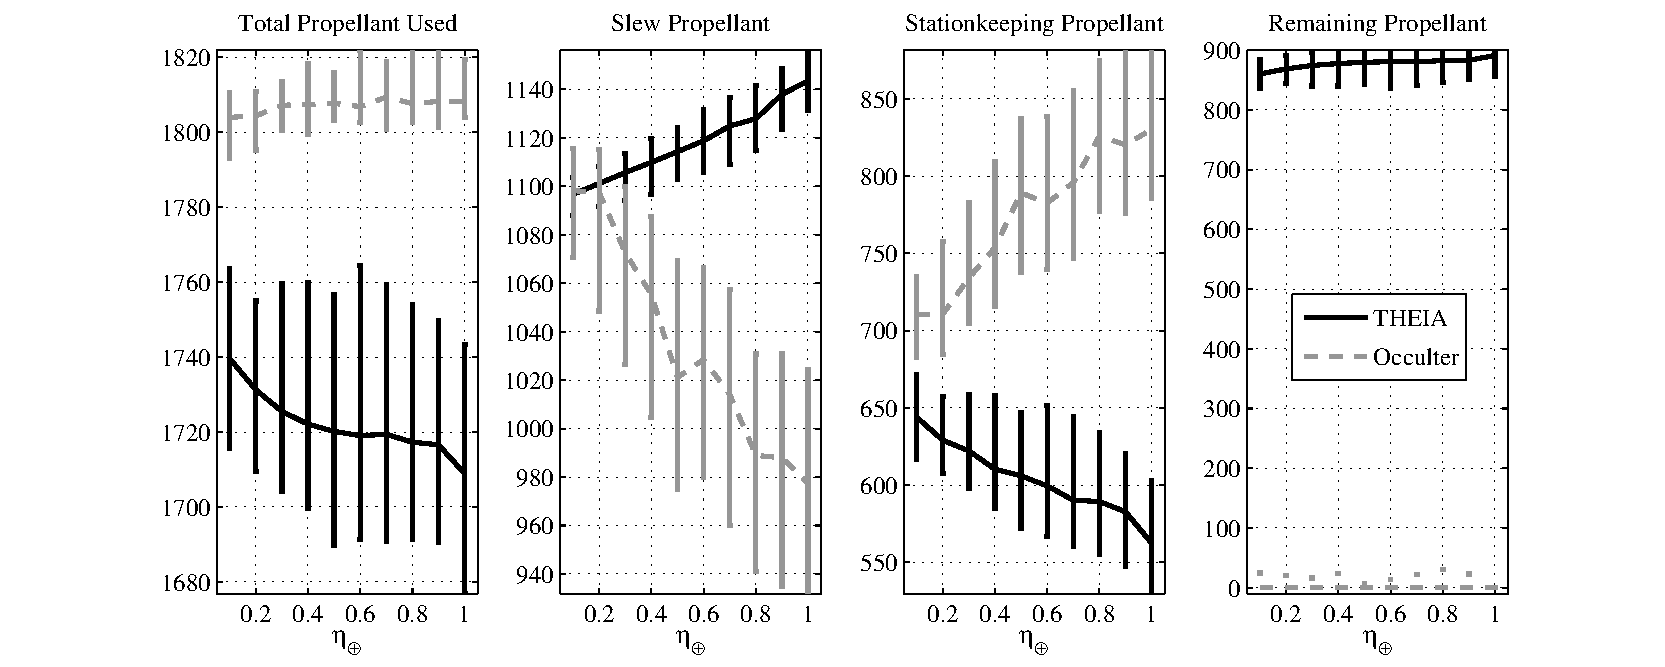
\includegraphics[width=0.9\columnwidth,clip=true,trim=0.8in 0in 0.75in 0in]{../figures/theiaFuel}
 \caption{Spacecraft propellant use (in kg).}
 \end{figure}
}
}

\subsection{Data Analysis}
\frame{
\frametitle{State Estimation}
\begin{itemize}
\item Any exosystem measurement is a partial observation of an underlying dynamical system
\[\Z_k = \boldsymbol{h}_k(\X_k,k) + \boldsymbol{n}\]
\item The system evolves via known physical laws
\[\X_{k+1} = \boldsymbol{f}(\X_k,k)\]
\item State estimation seeks to reconstruct the full state
\[ \hat\X_k = \arg\min E\{\Vert \X_k - \hat\X_k\Vert^2\} \]
\item Can be formulated as a recursive two-step process:
\[ p(\X_k | \Z_{1:k-1}) = \int p(\X_k | \X_{k-1})p(\X_{k-1} | \Z_{1:k-1}) d\X_{k-1} \]
\[ p(\X_k|\Z_{1:k}) = \frac{p(\Z_k | \X_k) p(\X_k | \Z_{1:k-1})}{p(\Z_k | \Z_{1:k-1})} \]
\end{itemize}
}

\frame{
\frametitle{Combining Data Sets}
  \only<1>{
  \begin{figure}[ht]
 \begin{center}
  \begin{tabular}{ll}
   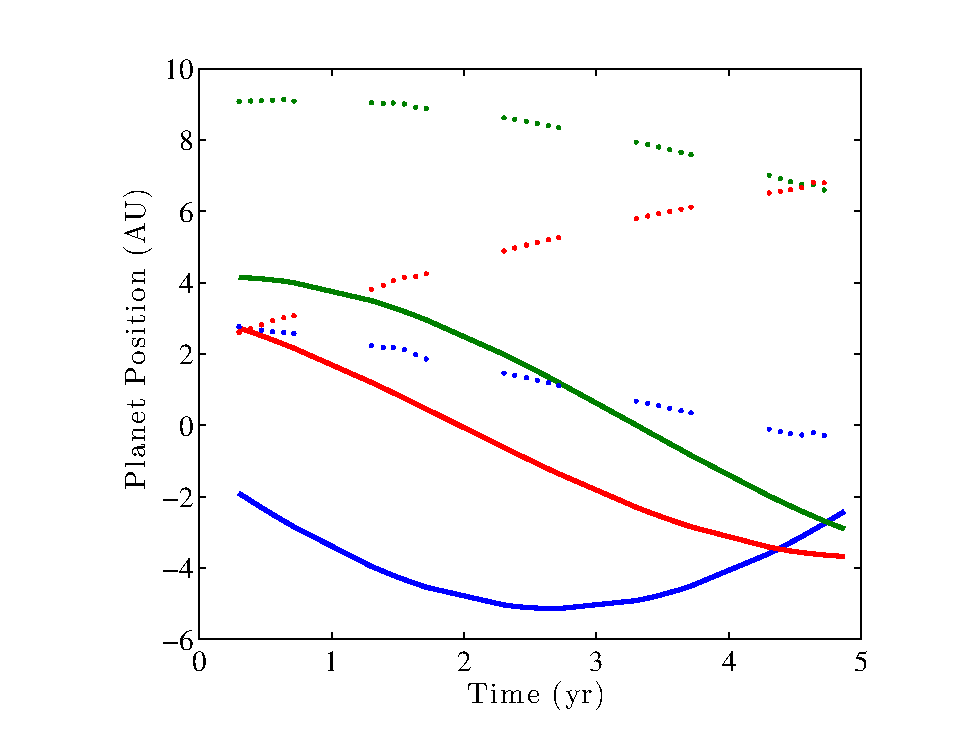
\includegraphics[height=5.25cm,clip=true,trim=0.6in 0in 0.1in 0in]{../figures/planpos1} &
    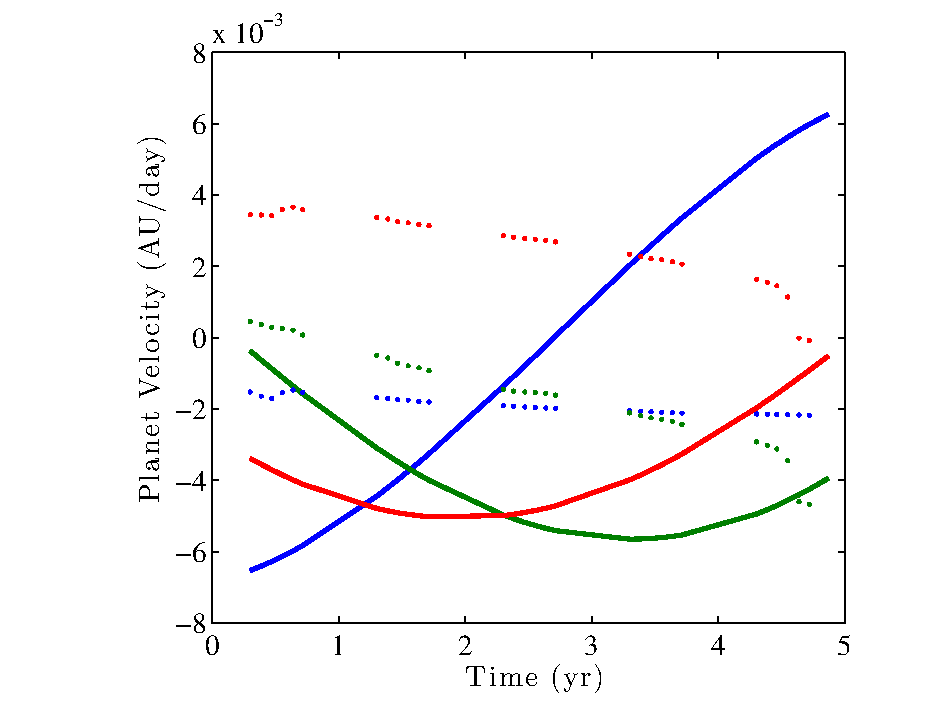
\includegraphics[height=5.25cm,clip=true,trim=0.9in 0in 0.1in 0in]{../figures/planvel1} 
     \end{tabular}
 \end{center}
\end{figure}
    }    
      \only<2>{
      \begin{figure}[ht]
 \begin{center}
  \begin{tabular}{ll}
   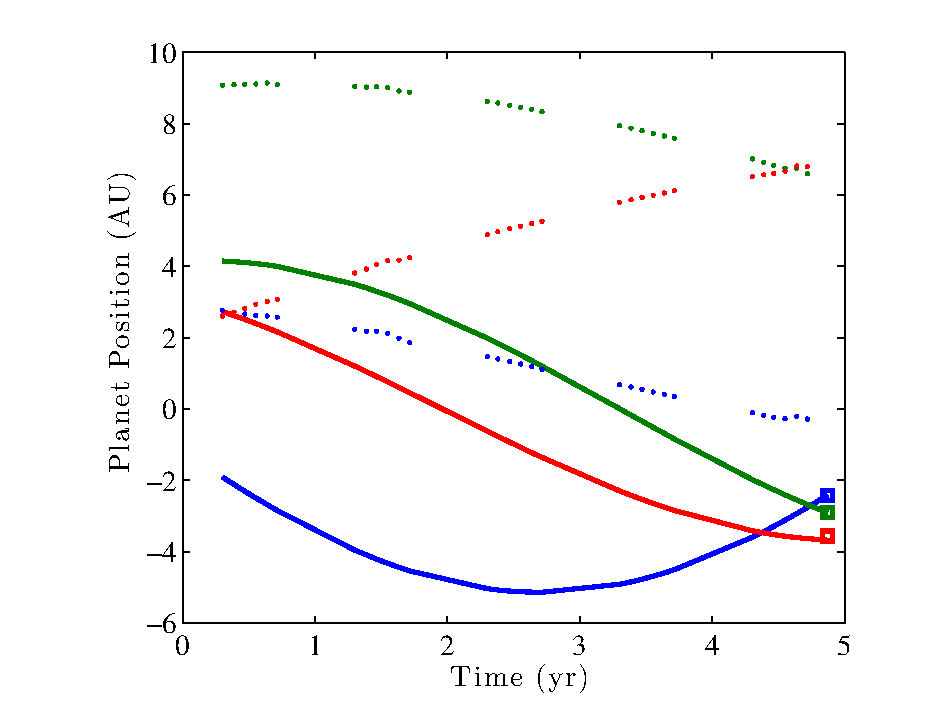
\includegraphics[height=5.25cm,clip=true,trim=0.6in 0in 0.1in 0in]{../figures/planpos2} &
    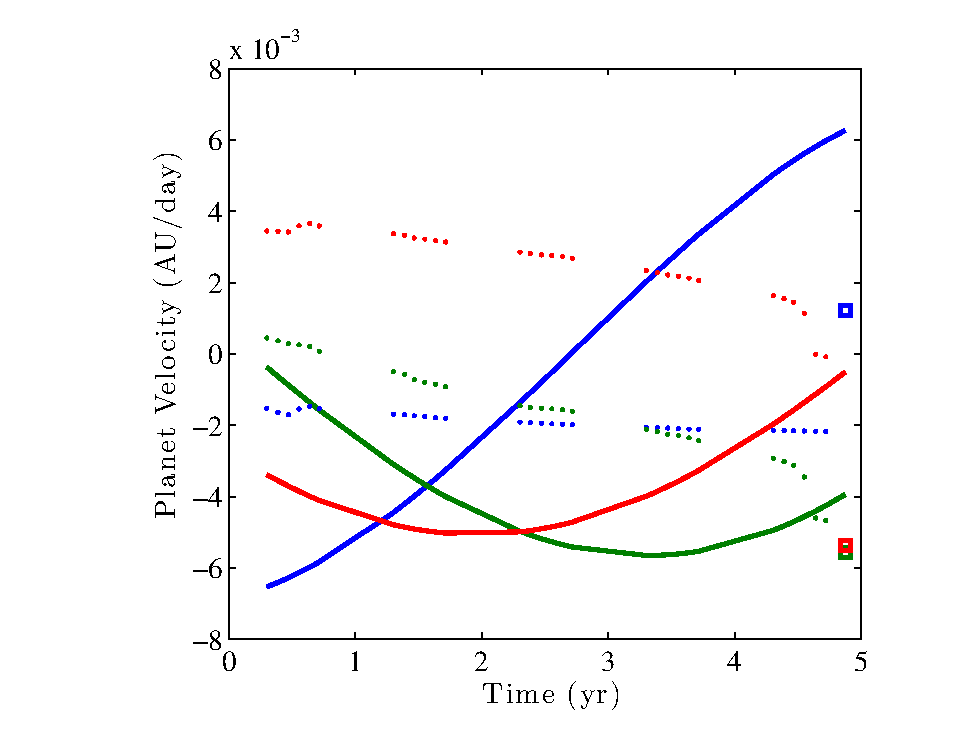
\includegraphics[height=5.25cm,clip=true,trim=0.9in 0in 0.1in 0in]{../figures/planvel2}
     \end{tabular}
 \end{center}
\end{figure} 
    }   
      \only<3>{
      \begin{figure}[ht]
 \begin{center}
  \begin{tabular}{ll}
   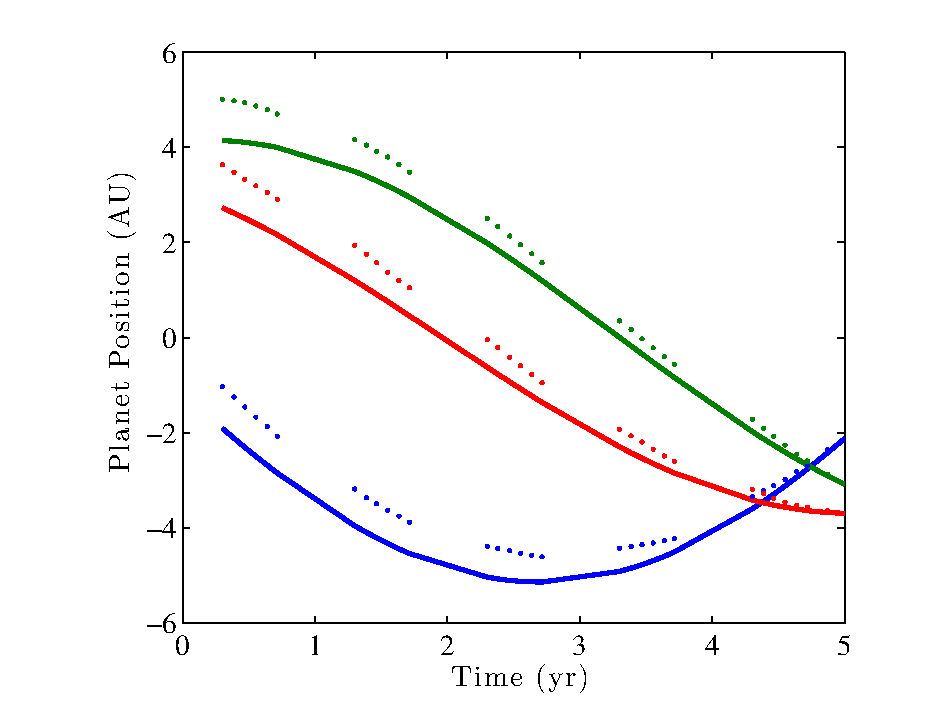
\includegraphics[height=5.25cm,clip=true,trim=0.6in 0in 0.1in 0in]{../figures/planpos3} &
    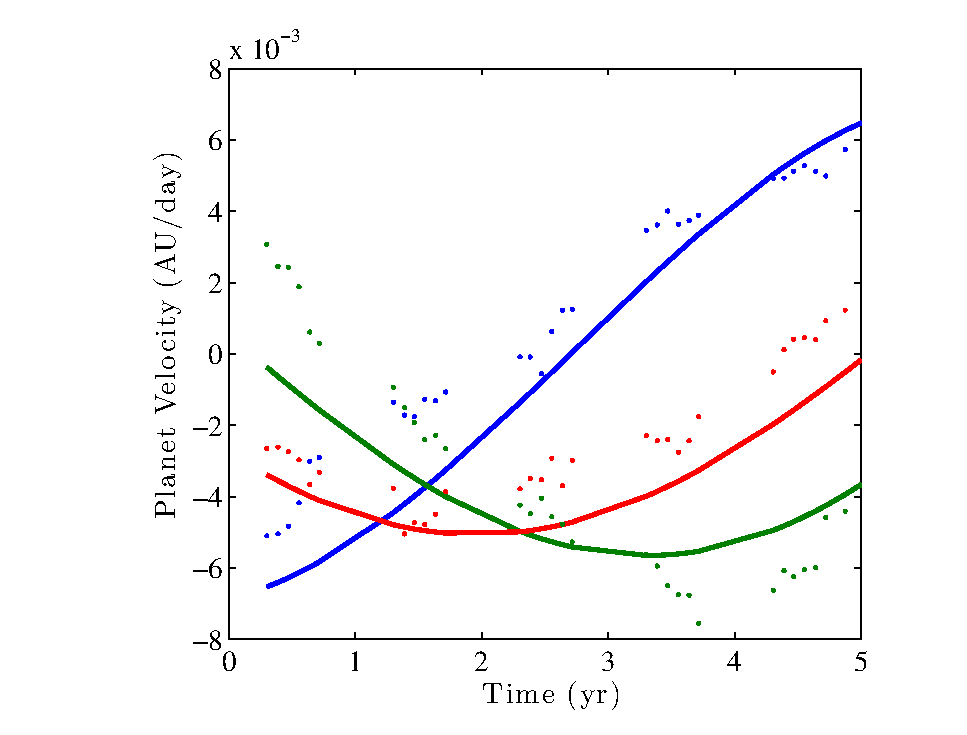
\includegraphics[height=5.25cm,clip=true,trim=0.9in 0in 0.1in 0in]{../figures/planvel3} 
     \end{tabular}
 \end{center}
\end{figure}
    }
    True state values (solid) and filter estimates (dotted) for $x$ (blue) $y$ (green) and $z$ (red) components of position and velocity.  
}

\section*{}
\subsection*{}
\frame{
\frametitle{Conclusions}
\begin{itemize}
\item Detailed exosystem and instrument modeling is very important to all aspects of planet-finding
\begin{itemize}
\item Mission design
\item Survey design
\item Data analysis
\end{itemize}
\item Statistical analyses can provide powerful tools for planning and data processing
\item Optimal estimation techniques are highly applicable to this area
\end{itemize}
}

\BackgroundPicture{backgrnd1}{1}{1}
\frame{
\frametitle{Thanks! }
	\begin{center}
\textbf{{Many, many thanks to:}}
	\bigskip	
	\begin{columns}[t]
	\column{0.3\columnwidth}
	\textbf{Jeremy Kasdin\\
	Bob Vanderbei\\
	Rob Stengel\\
	Ed Turner\\
	Michael Littman}
	
	\column{0.3\columnwidth}
	\textbf{Laurent Pueyo\\
	Eric Cady\\
	Tyler Groff\\
	Stephanie Goldfarb\\
	Don Lindler}
	
	\column{0.3\columnwidth}
	\textbf{Melanie Savransky\\
	Mac Haas\\
	Candy Reed\\
	Jessica O'Leary\\
	Jill Ray}

	\end{columns}
	\bigskip
	\textbf{{and the whole TPF (now HCIL) group!}}
	
	\end{center}
}
\setbeamertemplate{background}{ \setbeamercolor{normal text}{bg=white} }

\appendix

\newcounter{finalframe}
\setcounter{finalframe}{\value{framenumber}}

\frame[allowframebreaks]{
\frametitle{References}
\setbeamerfont{refs}{size=\tiny} 
\usebeamerfont{refs}
\bibliography{Main}   
\bibliographystyle{apalike}   
}


\section{Backup Slides}

\subsection{Known Exoplanet Statistics}
\frame{
\frametitle{Current Exoplanet Statistics}
\only<1>{\begin{figure}[ht]
    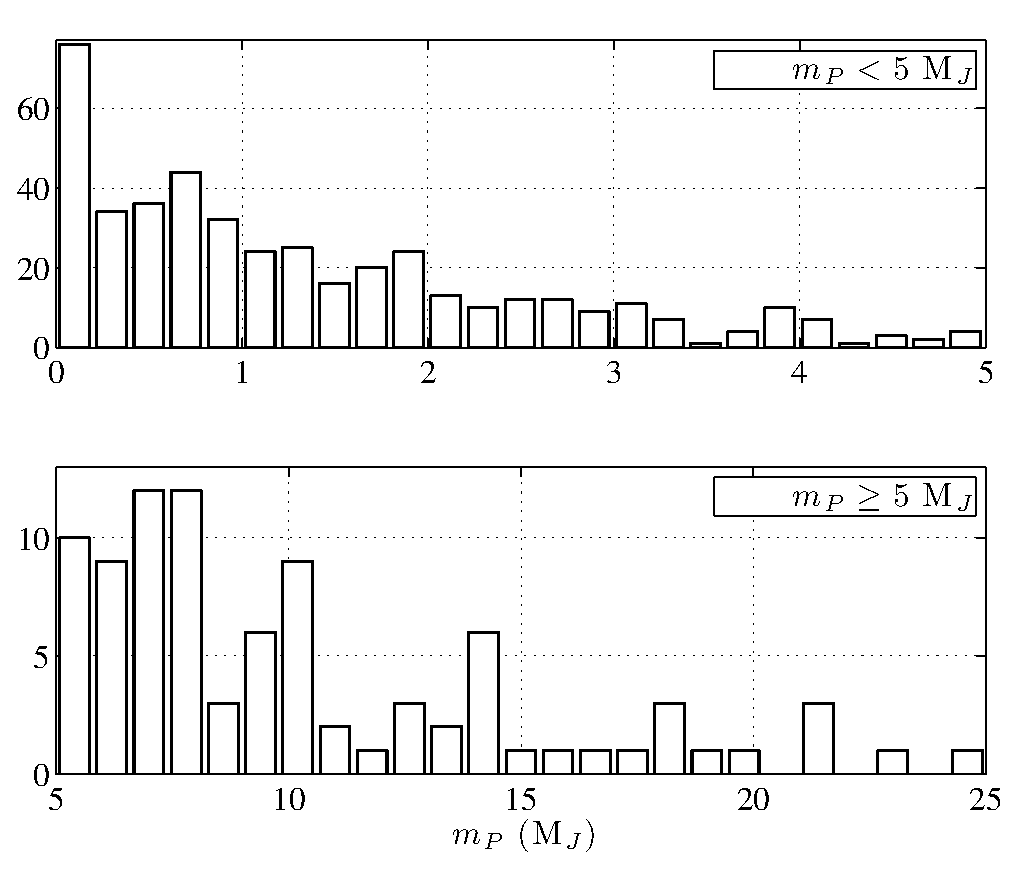
\includegraphics[width=0.48\columnwidth]{currMassHist}
    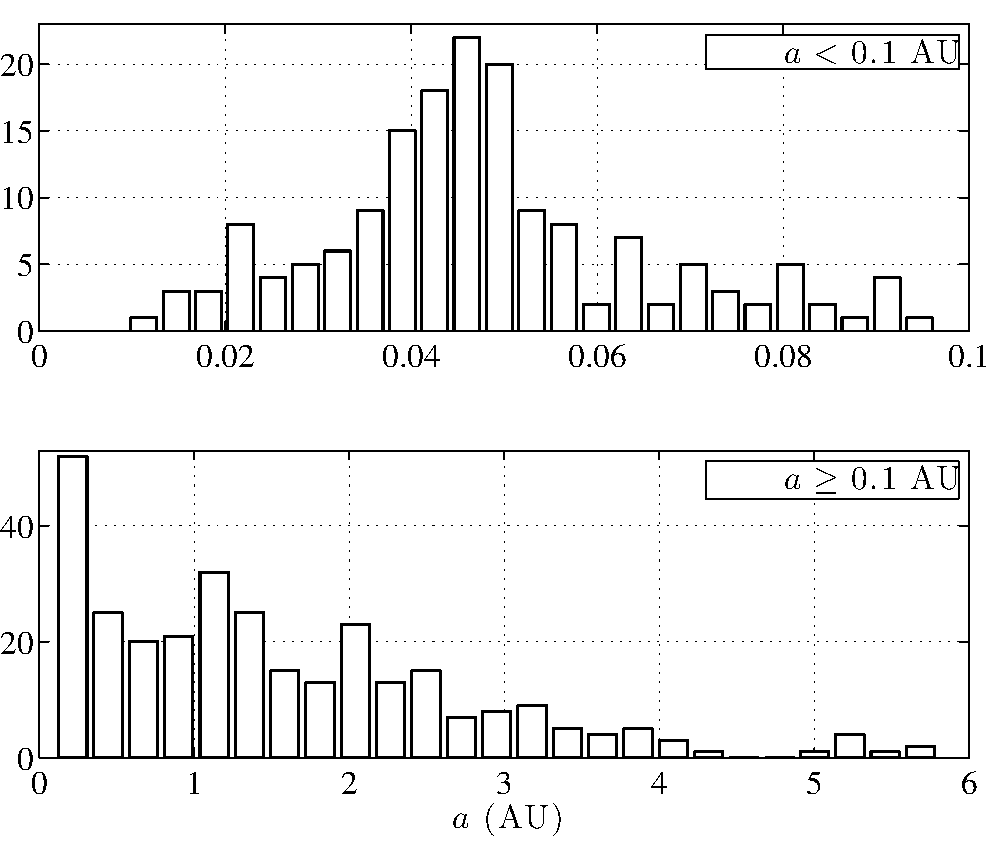
\includegraphics[width=0.48\columnwidth]{currSMaxHist}
\end{figure}}
\only<2>{\begin{figure}[ht]
    \includegraphics[width=0.48\columnwidth]{M_v_a}
    \includegraphics[width=0.48\columnwidth]{e_v_a}
\end{figure}}
\begin{center}
Data from \url{http://nsted.ipac.caltech.edu/}. Retrieved 06/01/2011.
\end{center}
}

\subsection{Keplerian Orbits}
\frame{
\frametitle{Keplerian Orbits}
\begin{figure}
	\begin{center}
	\includegraphics[width = 0.6\columnwidth]{../figures/anomaly_diagram}
	\end{center}
\end{figure}
}

\subsection{Imaging Systems and Space Observatories}
\frame{
\frametitle{Starlight Suppression}
\vspace{-4ex}
\begin{columns}[t]
\column{0.35\columnwidth}
\begin{figure}
	\begin{center}
	\includegraphics[width=1\columnwidth]{pupilPSF}
	\caption{Open aperture PSF.}
	\end{center}
\end{figure}

Two basic options: internal or external suppression system (with lots of variations).  

\column{0.35\columnwidth}
\begin{figure}
	\begin{center}
	\includegraphics[width=1\columnwidth]{ripplePSF}
	\caption{Pupil mask PSF.}
	\end{center}
\end{figure}
\vspace{-4ex}
\begin{figure}
	\begin{center}
	\includegraphics[width=0.75\columnwidth]{pupil_mask}
	\caption{Open aperture PSF.}
	\end{center}
\end{figure}

\column{0.35\columnwidth}
\begin{figure}
	\begin{center}
	\includegraphics[width=1\columnwidth]{theiaPSF}
	\caption{Apodized Pupil PSF.}
	\end{center}
\end{figure}
\vspace{-5ex}
\begin{figure}
	\begin{center}
	\includegraphics[width=0.75\columnwidth]{../figures/theiaOcculter}
	\caption{Apodized Pupil PSF.}
	\end{center}
\end{figure}
\end{columns}
}


\frame{
\frametitle{Imaging Constraints}

\begin{figure}
	\begin{center}
	\includegraphics[width=0.3\columnwidth]{../figures/keepoutZones}
	\hspace{1cm}
	\includegraphics[width=0.55\columnwidth]{../figures/halo_orbit}
	\end{center}
\end{figure}
\begin{block}{}
Star observability is determined by spacecraft orbit and time of year.
\end{block}
}


\subsection{Derivation of Lambert Phase Function}
\frame{
\frametitle{Derivation of Lambert Phase Function}
\framesubtitle{\cite{sobolev}}
\begin{columns}
	\column{0.4\columnwidth}
	\begin{figure}
		\begin{center}
		\includegraphics[width=1\columnwidth]{../figures/reflection_diagram}
		\end{center}
	\end{figure}
	
	\column{0.6\columnwidth}  
	Let $(\alpha, \delta)$ be the planetary latitude and longitude, $\mu$ the angle of incident radiation, $\gamma$ the angle of emergent radiation at a surface point, and $\xi$ the azimuthal angle between them:
	\begin{eqnarray*}
		\cos\mu &=& \cos\alpha \cos(\beta - \delta) \triangleq C_\mu\\
		\cos\gamma &=& \cos\alpha \cos\delta \triangleq C_\gamma\\
		\cos\beta &=& \cos\mu\cos\gamma - \sin\mu\sin\gamma\cos\xi
	\end{eqnarray*}
	The emergent intensity is given by $I = C_\gamma F \rho(C_\mu,C_\gamma,\xi)$ where $\pi C_\gamma F$ is the flux on a patch of the surface and $\rho$ is the reflection coefficient.
\end{columns}
The energy crossing a surface patch into unit solid angle is $C_\gamma C_\mu F \rho dA$ where $dA = R_p^2 \cos\alpha d\alpha d\delta$.
}

\frame{
\frametitle{Derivation of Lambert Phase Function (contd.)}
\framesubtitle{\cite{sobolev}}
So, the energy per second per unit area per unit solid angle received by an observer is:
\begin{equation*}
E(\beta) = \frac{F R_p^2}{d^2} \int_{\beta - \pi/2}^{\pi/2} \cos(\beta - \delta) \cos\delta d\delta  \int_{-\pi/2}^{\pi/2} \rho(C_\mu,C_\gamma,\xi) \cos^3 \alpha d\alpha 
\end{equation*}
The phase function is defined as the ratio of $E(\beta)/E(0)$.  For isotropic scattering, $\rho$ is constant so:
\begin{equation*}
\phi_L(\beta) = \frac{\int_{\beta - \pi/2}^{\pi/2} \cos(\beta - \delta) \cos\delta d\delta}{ \int_{-\pi/2}^{\pi/2} \cos(-\delta) \cos\delta d\delta} = \frac{\sin(\beta)+(\pi-\beta)\cos(\beta)}{\pi}
\end{equation*}
}

\subsection{Mapping of Instruments to Parameter Set}
\frame{
\frametitle{Imaging}
\framesubtitle{\cite{kasdin2006,savransky2010}}
\begin{itemize}
 \item Model observation as:
   \begin{equation*}
   \mathbf{z}(x,y) = C_p\bar P(x - \xi,y - \eta) +\boldsymbol{n}
   \end{equation*}
   where $C_p$ is the mean photon count at planet location - pixel $(\xi,\eta)$, $\bar P$ is the normalized PSF, and $\boldsymbol{n}$ is the noise.
\item Pixel location maps to on-sky separation as:
\[ \mathbf{s} = \leftexp{\mathcal{I}}{C}^{\mathcal{S}} \left[\begin{array}{c} \xi \\ \eta \end{array}\right] \frac{\sqrt{\Delta \alpha}}{f\varpi} \]
where $\Delta \alpha$ is the physical pixel size, $f$ is the focal length, and $\leftexp{\mathcal{I}}{C}^{\mathcal{S}}$ rotates the sky frame into the inertial frame.
\item $C_p \propto F_P$, with constant depending on camera characteristics.
\end{itemize}
}

\frame{
\frametitle{Transit Photometry}
\framesubtitle{\cite{mandel2002analytic}}
\vspace{-1ex}
\begin{figure}[ht]
 \begin{center}
    \includegraphics[width=0.35\columnwidth]{../figures/phot_model}
 \end{center}
\end{figure}
\vspace{-2ex}
\[ \frac{F^{(e)}}{F} = 
\left\{ \begin{array}{l l}
1 & R_S + R < s\\
1 - \frac{1}{\pi} \left[ \frac{R^2 }{R_S^2}\kappa_0 + \kappa_1 - \sqrt{\frac{s^2}{R_S^2} - \frac{\left( R_S^2 + s^2 - R^2\right)^2}{4 R_S^4}}\right] & \vert R_S - R \vert < s \le R_S + R \\
1 - \left(\frac{R}{R_S}\right)^2 & s \le R_S - R\\
0 & s \le R - R_S
\end{array} \right. \]
\[ \kappa_0 = \cos^{-1}\left(\frac{R^2 +s^2 - R_S^2}{2Rs}\right) \qquad \kappa_1 =  \cos^{-1}\left(\frac{R_S^2 - R^2 + s^2}{2R_S s}\right) \]
}

\frame{
\frametitle{Doppler Spectroscopy}
\framesubtitle{\cite{marcy1992precision,butler1996attaining}}
\begin{itemize}
\item The observed spectrum as a function of wavelength:
\[
I_{obs}(\lambda) = \kappa \left[ I_S(\lambda + \Delta\lambda_S)T_C(\lambda + \Delta\lambda_C) \right] \otimes \PSF
\]
where $I_S$ is the stellar spectrum and $T_C$ is the transmission function of the absorption cell.
\item After deconvolution and fitting, relate to parameter set via relativistic Doppler equation:
\[
\frac{\Delta\lambda_S - \Delta\lambda_C}{\lambda} = \frac{\left(1 + \left(\frac{v}{c}\right)^2\cos\theta\right)\left(1 + \rho_g\right)}{n\sqrt{1 - \left(\frac{v}{c}\right)^2}} - 1
\]
where $v = \Vert \Rd_{S/sc}\Vert$ and $\cos\theta = \frac{{\mf r}_{S/sc}}{\Vert \R_{S/sc}\Vert}  \cdot \frac{\Rd_{S/sc}}{\Vert\Rd_{S/sc}\Vert}$
\end{itemize}
}

\frame{
\frametitle{Interferometric Astrometry}
\framesubtitle{\cite{konacki2002frequency,savransky2010simulation}}
Narrow-angle astrometric measurement with interferometer baseline $B$:
\vspace{-3ex}
\begin{columns}
\column{0.5\columnwidth}
\begin{figure}
\centering
\includegraphics[width=0.9\columnwidth]{../figures/narrow_angle_model}
\end{figure} 
\column{0.5\columnwidth}
\begin{align}
d_i &=B \left(\cos\theta_i - \cos(\theta_i - \Delta\theta_i)\right) \nonumber\\
&=B\left(\cos\theta_i(1 - \cos\Delta\theta_i) - \sin\theta_i \sin\Delta\theta_i\right)\nonumber
\end{align}
\[
\mf d = B\left[ \begin{array}{l} \mf b_1 \cdot \left(\hat{\mf r}_{S/sc} - \hat{\mf r}_{c/sc}\right) \\\mf b_2 \cdot \left(\hat{\mf r}_{S/sc} - \hat{\mf r}_{c/sc}\right) \end{array}\right] + \mf n
\]
\end{columns}
\usebeamerfont{smalleq}
\begin{align*}
\hat\R_{S/sc} &= \frac{\R_{S/sc}}{\| \R_{S/sc} \|} = (\R_{S/O}(t_0) + \R_\mu +\Delta \R_{S/G}- \R_{sc/O})\times  \\
&\begin{array}{l}\left\{
\R_{S/O}(t_0)\cdot\R_{S/O}(t_0) + \R_\mu \cdot \R_\mu + \Delta \R_{S/G} \cdot \Delta \R_{S/G} +\R_{sc/O} \cdot \R_{sc} \right. \\
\;  {}+ 2\R_{S/O}(t_0) \cdot \R_\mu + 2\R_{S/O}(t_0) \cdot \Delta \R_{S/G} - 2\R_{S/O}(t_0) \cdot \R_{sc/O} \\
\; \left. {} + 2 \R_\mu \cdot \Delta \R_{S/G} - 2 \R_\mu \cdot \R_{sc/O} - 2 \Delta \R_{S/G} \cdot \R_{sc/O}\right\}^{-\frac{1}{2}} 
 \end{array}
\end{align*}
}

\subsection{Derivation of $\Delta$mag Extrema}
\frame{
\frametitle{Derivation of $\Delta$mag Extrema}
\framesubtitle{\cite{brown2004a}}
\usebeamerfont{smalleq}
The relative magnitude assuming a Lambert phase function is:
\begin{equation*}
	\Delta\textrm{mag} = -2.5\log\left(p \left(\frac{R}{r}\right)^2 \Phi(\beta)\right), \Phi = \frac{\sin(\beta)+(\pi-\beta)\cos(\beta)}{\pi},
\end{equation*}
where the phase angle is given by $\beta = \sin^{-1}\left(\frac{s}{r}\right)$.
So, for constant $p$, $R$ and $s$, the extrema of $\Delta$mag occurs when:
\begin{equation*}
\frac{\sin(\beta)}{\pi}\left[ 2\sin(\beta)\cos(\beta)+(\pi-\beta)\left(2\cos^2(\beta) - \sin^2(\beta)\right) \right] = 0
\end{equation*}
The maximum occurs when $\beta = 1.10473$, so the minimum $\Delta$mag as a function of $s$ is given by
\begin{equation*}
\Delta\textrm{mag}_{min} = -2.5\log\left(0.459455\frac{p_{max} R_{max}^2}{s^2}\right)
\end{equation*}
}

\frame{
\frametitle{Derivation of $\Delta$mag Extrema}
\usebeamerfont{smalleq}
The maximum value of $\Delta$mag for a fixed $s$ occurs when the planet is in front of the star, such that 
\begin{equation*}
\beta = \pi - \sin^{-1}\left(\frac{s}{r_{max}}\right)
\end{equation*}
where $r_{max} = a_{max}(1+e_{max})$.\\
Thus
\begin{equation*}
\Delta\textrm{mag}_{max} = -2.5\log\left(p_{min} R_{min}^2 \frac{s-\sqrt{r_{max}^2 - s^2}  \sin^{-1}\left(\frac{s}{r_{max}}\right)}{\pi r_{max}^3}\right)
\end{equation*}
}

\subsection{Distributions of Keplerian Parameters}
\frame{
\frametitle{The Distribution of $\nu$}
\usebeamerfont{smalleq}
\begin{itemize}
\item Let $\nu = g(M,e)$ and $M = h(\nu,e)$ with $f_{\bar{e}}$ the probability density function of $\bar{e}$.  The cumulative distribution function of $\bar{\nu}$ is:
\[F_{\bar{\nu}}(\nu) = P(g(\bar{M},\bar{e}) \le \nu) = \int_{-\infty}^{\infty} P(g(\bar{M},e) \le \nu | \bar{e} = e)f_{\bar{e}}(e)\, \mathrm{d}e\]

\item $\bar{M}$ and $\bar{e}$ are independent and $e \in [0,1]$ so:
\[F_{\bar{\nu}}(\nu) = \int_{0}^{1} P(\bar{M} \le h(\nu,e))f_{\bar{e}}(e)\, \mathrm{d}e\]
\end{itemize}	

\begin{block}{Probability Density Function of $\nu$}
	\[f_{\bar{\nu}}(\nu) =  \frac{\mathrm{d}}{\mathrm{d}\nu}F_{\bar{\nu}}(\nu) =  \frac{1}{2\pi} \int_{0}^{1} \frac{\partial h}{\partial \nu}f_{\bar{e}}(e)\, \mathrm{d}e  =  \frac{1}{2\pi} \int_{0}^{1} \frac{\left(1-e^2\right)^\frac{3}{2}}{\left(1+e\cos\nu\right)^2} f_{\bar{e}}(e)\, \mathrm{d}e\]
\end{block}
}

\frame{
\frametitle{The Distribution of Apparent Separation}
\begin{itemize}
\item $s \approx r \sin \beta$

\item Let $\bar l = \sin\bar\beta$
\[
f_{\bar l}(l) = f_{\bar \beta}(\sin^{-1}(l)) \left| \frac{ \mathrm{d}}{ \mathrm{d} l} \sin^{-1}(l) \right| = 
\left\{
    \begin{array}{l l}
    \frac{l}{\sqrt{1 - l^2}} & l \; \in \; [0,1) \\
    0 & \mathrm{else} \end{array}\right.
\]
\item Since $\bar s = \bar r \bar l$
\[f_{\bar{s}}(s) = \int_{-\infty}^\infty \frac{1}{l} f_{\bar{r}}\left(\frac{s}{l}\right)f_{\bar{l}}(l)\, \mathrm{d}l \]
\end{itemize}
\vspace{-1ex}
\begin{block}{Probability Density Function of $s$}
\[f_{\bar s}(s) = \frac{1}{\pi}  \int_{0}^1 \int_{0}^{\infty} \int_{0}^{1} \frac{s}{a\sqrt{\left(1 - l^2\right)\left[(ael)^2 - (al-s)^2\right]}}f_{\bar{e}}(e) \, \mathrm{d}e \, f_{\bar{a}}(a)\, \mathrm{d}a \, \mathrm{d}l  \]
\end{block}
}


\frame{
\frametitle{Distributions of Keplerian Orbital Elements}
\framesubtitle{\cite{savransky2011parameter}}
\[f_{\bar{\nu}}(\nu) =  \frac{1}{2\pi} \int_{0}^{1} \frac{\left(1-e^2\right)^\frac{3}{2}}{\left(1+e\cos\nu\right)^2} f_{\bar{e}}(e)\, \mathrm{d}e\]
\[f_{\bar{r}}(r) = \frac{1}{\pi}\int_{0}^{\infty} \int_{0}^{1} \frac{r}{a\sqrt{(ae)^2 - (a-r)^2}}f_{\bar{e}}(e) \, \mathrm{d}e \, f_{\bar{a}}(a)\, \mathrm{d}a \]
\[f_{\bar s}(s) = \frac{1}{\pi}  \int_{0}^1 \int_{0}^{\infty} \int_{0}^{1} \frac{s}{a\sqrt{\left(1 - l^2\right)\left[(ael)^2 - (al-s)^2\right]}}f_{\bar{e}}(e) \, \mathrm{d}e \, f_{\bar{a}}(a)\, \mathrm{d}a \, \mathrm{d}l \]
\[f_{\bar F_R}(F_R) = \int\limits_{-\infty}^\infty \frac{f_{\bar{n}}(n)}{npR^2} \cos\left(\sum_{k=1}^{\infty} b_k \left(\frac{F_R}{npR^2} - \frac{1}{\pi}\right)^k\right)\left|\sum_{k=1}^\infty k b_k \left(\frac{F_R}{npR^2} - \frac{1}{\pi}\right)^{k-1} \right| \, \mathrm{d}n \]
\[b_k = \frac{1}{k \alpha_1^k} \sum_{x \in X} (-1)^{\vert x \vert} \prod_{r=1}^{\vert x\vert}(k-1+r)  \prod_{i=1}^{k-1}\frac{\left(\alpha_{i+1}/\alpha_1\right)^{x_i}}{x_i!}\]
}

\subsection{Optimal Cadence for Transits}
\frame{
\frametitle{Transit Probability}
\begin{itemize}
\item Transits occur when
\[s < R_S + R \]
so probability of transit is 
\[ P(s < R_S + R) = \int_0^{R_S + R} f_{\bar s} (s) \intd{s} \]
\item Assuming a specific observing cadence, occurrence of transits is modeled as a Poisson process.  In each time interval $\Delta t$, the probability of transits is
\[ P[N_{\textrm{transits}}(\Delta t) > 0] = 1 - e^{-\lambda \Delta t}  \]
\item To capture all transits of orbits with semi-major axis $a_0$ in one orbital period
\[ \Delta t \le  \frac{1}{\pi} \frac{R_s + R}{a_0} \]
\end{itemize}
}

\frame{
\frametitle{Transit Detection}
\vspace{-2ex}
\begin{figure}[ht]
\centering
\includegraphics[width=0.65\columnwidth]{../figures/transitCadences}
\vspace{-2ex}
\caption{Portion of observable transits detected over one orbital period for $a_0 = 1, R_S = R_\odot$ and $R = 0$ as a function of observation cadence using Monte Carlo (black) and algebraic solution (green).}
\end{figure} 
}

\subsection{Dynamic Filtering}
\frame{
\frametitle{Dynamic Filtering (The Optimal Estimation Way)}
\begin{itemize}
\item Measurements ($\Z$) at time $k$ are a function of a state vector ($\X$) describing the positions of all orbiting planets, and time, with added noise $\boldsymbol{n}$ of covariance $R$:
\begin{equation*}
\Z_k = \boldsymbol{f}(\X_k,k) + \boldsymbol{n}
\end{equation*}
\item The solution to this problem is a minimization with respect to $\X$ for $N$ observations of the cost function:
\begin{equation*}
J = \sum_{k=1}^N \left[\Z_k - \boldsymbol{f}(\X_k,k)\right]^T R^{-1}  \left[\Z_k - \boldsymbol{f}(\X_k,k)\right]
\end{equation*}
subject to the constraints of the physical system (i.e. Newtonian dynamics) and any inherent constraints in the formulation of the state (i.e., quaternion definition, eccentricity bounds, etc.).
\item Can be re-formulated as a recursive filter
\end{itemize}
}

\frame{
\frametitle{Dynamic Filtering (The Bayesian Way)}
\begin{itemize}
\item Assume a Markov process with state $\X$ and observation $\Z$.  Then
\[ p(\X_0,\X_1\cdots \X_n, \Z_1,\Z_2 \cdots \Z_n) = p(\X_0) \prod_{j = 1}^{n} p(\Z_j | \X_j)p(\X_j | \X_{j-1}) \]
\item Predict the next state given the observed history
\[ p(\X_j | \Z_{1:k-1}) = \int p(\X_j | \X_{j-1})p(\X_{j-1} | \Z_{1:j-1}) d\X_{j-1} \]
\item Update the state estimate given the current observation
\[ p(\X_j|\Z_{1:j}) = \frac{p(\Z_j | \X_j) p(\X_j | \Z_{1:j-1})}{p(\Z_j | \Z_{1:j-1})} \]
\end{itemize}
}

\frame{
\frametitle{Extended Kalman Filter}
\begin{equation*}
\begin{array}{ll}
\mathbf{\dot{\hat{x}}}(t) = \mathbf{f}(\mathbf{\hat{x}}(t),t) \qquad \qquad &
\mathbf{\dot{P}}(t) = \mathbf{F}(t)\mathbf{P}(t)+\mathbf{P}(t)\mathbf{F}^T(t) + \mathbf{Q} \\
\mathbf{\hat{x}}_0 = E[\mathbf{x}(0)] &
\mathbf{P}_0 = E[(\mathbf{x}(0) - \mathbf{\hat{x}}_0)(\mathbf{x}(0) - \mathbf{\hat{x}}_0)^T] \\
\mathbf{F}(t) = \left. \frac{\partial \mathbf{f}}{\partial \mathbf{x}}\right|_{\mathbf{\hat{x}}(t)} & 
\mathbf{Q}(t) = E[\mathbf{w}(t) \mathbf{w}^T(\tau)] 
\end{array}
\end{equation*}
 
\begin{equation*}
\begin{array}{l}
\mathbf{\hat{x}}^+_{k_i} = \mathbf{\hat{x}}^-_k + \mathbf{K}_{k_i}\left(\mathbf{y}_k -  \mathbf{h}(\mathbf{\hat{x}}^+_{k_{i-1}}) -   \mathbf{H}_{k_i} (\mathbf{\hat{x}}^-_k  -  \mathbf{\hat{x}}^+_{k_{i-1}})\right) \qquad \mathbf{\hat{x}}^+_{k_{0}} = \mathbf{\hat{x}}^-_{k}\\
\mathbf{K}_{k_i} = \mathbf{P}^-_k \mathbf{H}^T_{k_i} \left(\mathbf{H}_{k_i} \mathbf{P}^-_k \mathbf{H}^T_{k_i} + \mathbf{R}_{k}\right)^{-1} \hfill \mathbf{H}_{k_i} = \left. \frac{\partial \mathbf{h}}{\partial \mathbf{x}}\right|_{\mathbf{\hat{x}}^+_{k_i}} \\
\mathbf{P}^+_{k_i} = \left(\mathbf{I} -  \mathbf{K}_{k_i}\mathbf{H}_{k_i}\right)\mathbf{P}^-_k \hfill
\mathbf{R}(t) = E[\mathbf{v}(t) \mathbf{v}^T(\tau)] 
\end{array} 
\end{equation*}

Various enhancements include:
\begin{itemize}
\item Simultaneous integration of state and covariance
\item Iteration on nonlinear observer functions
\item Introduction of inequality state constraints 
\end{itemize}
}

\frame{
\frametitle{EKF Modifications}
\begin{itemize}
\item Position and Velocity state makes it easy to describe open orbits
\begin{itemize}
\item Introduce inequality constraints of the form $D \bar{X} \le d$ to constrain orbital specific energy
\item At each time step, solve quadratic programming problem of the form $\min_{\tilde{x}} \left(\tilde{x}^TW\tilde{x} - 2\bar{X}^TW\tilde{x} \right)$ s.t.  $D \tilde{x} \le d$ \cite{simon2006}
\end{itemize}

\item Nonlinearities in state propagation make filter very sensitive to initial conditions
\begin{itemize}
\item Attempt to constraint initial conditions via periodograms and other coarse analysis of data
\item Introduce random restarts when state or covariance diverges
\end{itemize}

\item Covariance estimate extrapolation is potential source of problems for nonlinear state update
\begin{itemize}
\item Evaluated particle filter-like approach 
\item Generate set of random states distributed according to current covariance estimate with mean of current state
\item Propagate random states and find covariance
\end{itemize}

\end{itemize}
}

\frame{
\frametitle{Priming Initial State with Update Step}
\begin{itemize}
\item We can use our initial measurement to improve the initialization step
\item For example, use formalism of the unscented transform to define the initial state:
\[\hat\X_0 = XWY^T\left(YWY^T + R\right)^{-1}\left(\Z_0 - Yw\right) \]
where
\[X = c [\mathbf{0} \quad A \quad -A] \]
\[Y = \boldsymbol{h}(\X,0) \]
and $c, w$ and $W$ are matrices of weights determined by the expected noise, $R$ is the covariance of $\boldsymbol{n}$ and $A$ is the Cholesky decomposition of the expected state covariance.
\end{itemize}
}


\setcounter{framenumber}{\value{finalframe}}

\end{document}
